\chapter{$k$-\'algebras} \justifying
Sea $k$ un cuerpo, por ejemplo $\bb Q, \bb R, \bb C, \bb F_p = \modulo{\bb Z}{p\bb Z}$ con $p$ primo. 
Se define  la caracter\'istica de $k$ por el morfismo de anillos
    $$\bt \bb Z\rar & k \\[-5mm] n \rarmaps & 1+\overset{n)}{\cdots} + 1 = n\\[-5mm] -n \rarmaps & -(1+\overset{n)}{\cdots} + 1) \et$$
    $\ker f = \{0\}$ \'o $\ker f = n \cdot \bb Z$, entonces por el teorema de factorizaci\'on, si $\ker f = \{0\}$, $f$ es inyectiva, de forma que $\bb Z \hookrightarrow k$, de forma que $\bb Q \hookrightarrow k$, ambos como subcuerpos. Entonces $ch(k) = 0$ si $\bb Q \subseteq k$ es un subcuerpo.

    Cuando $\ker f = n \bb Z$, por el teorema de factorizaci\'on, 
    $$\bt \modulo{\bb Z}{n \bb Z} \rar{\bar f} & k  \et$$
    es un morfismo de anillos inyectivo, y $\modulo{\bb Z}{n \bb Z}$ es un subanillo de $k$, y es \'integro por serlo $k$. Y cuando $n = p$ primo, $ch(k) = p$. 

    Es decir, la caracter\'istica es el $p$ tal que $1+\overset{p)}{\cdots} + 1 = p =0$. 
\begin{defi}
    Una $k$-\'algebra es un anillo $(A,+,\cdot)$ que contiene a $k$ como subanillo. Es decir, que la suma y producto de $k\subset A$ es la de $A$. O como un morfismo inyectivo de $k$ en $A$. Tambi\'en podemos verlo como $(A,+)$ es un $k$-espacio vectorial $\lambda \in k, \, a\in  A \Rightarrow \lambda \cdot a \in A$
\end{defi}
\begin{ejem}
    $k[x_1,\ldots, x_n]$ es una $k$-\'algebra, donde $k \subset k[x_1,\ldots, x_n]$ son los polinomios de grado 0. 

    Si $X$ es un conjunto, $F(X) = \{f:X \longrightarrow k \text{ aplicaci\'on}\}$, que tiene estructura de anillo, 
    $$(f+g)(x) = f(x) + g(x) \qquad (f\cdot g)(x) = f(x) \cdot g(x)$$
    y contiene a $k$ pues para cada $\lambda \in k$, $h_{\lambda}$ funci\'on constante $\lambda$,
    $$h_{\lambda}(x) = \lambda \, \forall \, x\in X$$
\end{ejem}
\begin{defi}
    Sea $A$ una $k$-\'algebra, un ideal $I \subset A$ verifica ser $(I,+) \subset(A,+)$ es un subgrupo y que si $ax\in I \, \forall a\in A, \, x\in I$. 
\end{defi}\begin{ejem}
    $I = (a) = \{a\cdot b \, / \, b \in A\}$.
\end{ejem}
\begin{ejem}
    En $F(X)$, $x\in X$, $\m_x = \{f \in F(X) \, / \, f(x)=0\}$ es un ideal de $F(X)$. 
\end{ejem}
\begin{obs}
    $I\subset A$ un ideal en particular es un $k$-subespacio vectorial de $A$. 
\end{obs}
\begin{defi}
    El cociente de $A$ por $I$ es $\, \modulo{A}{I}$, el conjunto cociente de $A$ por la relaci\'on $a\sim b \iff a-b \in I$. Entonces $[a]=a+I$ y $(\modulo{A}{I}, +, \cdot )$ es $k$-\'algebra con 
    $$[a]+[b] = [a+b]\qquad [a]\cdot [b] = [a\cdot b]$$
\end{defi}
\section{Morfismos de $k$-\'algebras}
Sean $A, B$ dos $k$-\'algebras,
\begin{defi}
    $f: A \longrightarrow B$ es un morfismo de $k$-\'algebras si es un morfismo de anillos y de $k$-espacios vectoriales. Como $k \subset A$ y $k \subset B$, se debe verificar que $f|_k = Id$. Es decir, 
    \begin{itemize}
        \item $f(a+b) = f(a) +f(b) $
        \item $f(ab) = f(a)f(b)$
        \item $f(\lambda) = \lambda\, \forall \, \lambda \in k$ 
    \end{itemize}
    \end{defi}
    \begin{ejems}
        \begin{itemize}
            \item La proyecci\'on can\'onica $p : A \longrightarrow \modulo{A}{I}$ es un morfismo de $k$-\'algebras, con $p(a) = [a]$.
            \item En $F(X)$, $x\in X$, 
            $$ \bt p_x : F(X) \rar &  k\\[-5mm] f \rarmaps & f(x) \et$$
            el morfismo tomar valor en $x$ es un morfismo de $k$-\'algebras.
            \item Pensemos $k[x_1, \ldots, x_n]$ como funciones en $F(k^n)$, dado $p(x_1, \ldots, x_n)$ lo pensamos como 
            $$\bt p: k^n \rar & k \\[-5mm] (\lambda_1, \ldots, \lambda_n) \rarmaps & p(\lambda_1 , \ldots, \lambda_n) \et$$
            y es un morfismo de $k$-\'algebras, si $ch(k) = 0$.

            Consideremos el caso $k[x] \longrightarrow\ F(k) = \{ f: k \longrightarrow k\}$, si $k = \bb F_2 = \{0,1\}$, tenemos $p(x) = x^2-x$, pensado como funci\'on, 
            $$\bt p: \bb F_2 = \{0,1\} \rar & \{0,1\} \\[-5mm] 0 \rarmaps & p(0)=0^2-0=0 \\[-5mm] 1 \rarmaps & p(1)=1^2-1=0 \et$$
            es decir, $p \equiv 0$ es la funci\'on constante cero. Si el cuerpo no es finito, se demuestra que si dos polinomios coinciden en todos los elementos de $k$, son el mismo. As\'i $k[x]$ no se puede incluir en $\bb F_2$.
        \end{itemize}
    \end{ejems}
    Sea $A$ una $k$-\'algebra, $I\subset A$ un ideal
    \begin{defi}
        $I$ es un ideal maximal si no est\'a contenido en ning\'un ideal distinto del total, es decir, si $I\subset J \subset A$, entonces $I=J$ \'o $I=A$. 
    \end{defi}
    \begin{defi}
        $I$ es un ideal primo si $a\cdot b \in I$ entonces $a\in I$ \'o $b\in I$. 
    \end{defi}
    \begin{prop}
        $I\subset A$ es primo $\iff \modulo{A}{I}$ es \'integro.
    \end{prop}
    \begin{prop}
        $I\subset A$ es maximal $\iff \modulo{A}{I}$ es cuerpo.
    \end{prop}
    \begin{cor}
        Si $I$ es maximal, entonces $I$ es primo. Conlcuimos as\'i que siempre hay ideales primos. 
    \end{cor}
    \begin{ejem}
        La aplicaci\'on tomar valor $p_x$ en $x$, verifica que 
        $$\ker p_x = \{f\in F(X)\}= (f)_0$$ es un ideal maximal, y por tanto primo. Usando el teorema de factorizaci\'on, 
        $$\modulo{F(X)}{\ker p_x} \simeq \Im p_x = k$$
        es un cuerpo, luego $\ker p_x = \m_x$. 
    \end{ejem}
    \begin{defi}
        El espectro de $A$ es el conjunto $X=Spec \, A$ de los ideales primos de $A$. Es un espacio, pudiendo elegir funciones $A\longrightarrow F(X)$ generalmente inyectivas. As\'i, $X\subseteq Spec \, F(X)$, por la asignaci\'on $x\mapsto \mathfrak m_x$. 
    \end{defi}
    \section{Producto directo y tensorial}
    Dadas dos $k$-\'algebras $A_1,\, A_2$, 
    \begin{defi}
        Se define la $k$-\'algebra producto directo $A_1 \times A_2$ donde para $\lambda \in k$, $\lambda(a_1,a_2) = (\lambda a_1, \lambda a_2)$.
    \end{defi}
    \begin{defi}
        Se define en el producto directo la proyecci\'on can\'onica
        $$\bt A_1 \times A_2 \rar{\pi} & A_1\\[-5mm] (a_1,a_2) \rarmaps & a_1 \et$$
        que es morfismo de $k$-\'algebras.
    \end{defi}
    \begin{defi}
        Se define el producto tensorial de $A_1$ y $A_2$ como el anillo
        $$A_1 \underset{k}{\otimes} A_2 = \{a_1 \otimes b_1 + a_2 \otimes b_2 + \cdots + a_s\otimes b_s \, / \, a_i \in A_1, \, b_j \in A_2 \}$$
    \end{defi}
    \begin{obs}
        Como en particular son espacios vectoriales,
        $$E \underset{k}{\otimes} E' = \sum_{1 \leq j \leq k, 1\leq j \leq s} e_i \otimes v_j \qquad e_i \in E, \, v_k \in E'$$
        siendo $\{e_i\}$ base de $E$ y $\{v_j\}$ base de $ E'$, luego $\{e_i \otimes v_j\}$ es base de $E \underset{k}{\otimes} E'$.
    \end{obs}
    \begin{prop}
        $A_1 \underset{k}{\otimes} A_2$ es $k$-\'algebra, con las operaciones
        $$(a_1 \otimes a_2) \cdot (a_1' \otimes a_2') = (a_1 \cdot a_1') \otimes (a_2 \cdot a_2') \qquad \lambda (a\otimes b) = \lambda a \otimes  b = a \otimes \lambda b$$
        que funciona como un producto
        $$a\otimes (b_1+ b_2) = a\otimes b_1 + a \otimes b_2 \qquad (a_1 + a_2) \otimes b = a_1\otimes b + a_2\otimes b$$
    \end{prop}
    \begin{defi}
        Se tienen los morfismos de anillos
        $$\bt A_1 \rar & A_1 \underset{k}{\otimes} A_2 \\[-5mm] a \rarmaps & a\otimes 1 \et$$
        $$\bt A_2 \rar & A_1 \underset{k}{\otimes} A_2 \\[-5mm] b \rarmaps & 1\otimes b \et$$
        luego nos deja multiplicar elementos provenientes de $A_1$ con provenientes de $A_2$:
        $$(a\otimes 1) \cdot (1 \otimes b) = a\otimes b$$
    \end{defi}
    \begin{ejem}
        Escojamos $k[x]$, de forma que $k[x] \underset{k}{\otimes} B \simeq B[x]$ con el isomorfismo natural
        $$\bt \sum \lambda_i x^i \otimes b =  \sum \lambda(x^i \otimes b) \rar & \sum_i b \lambda_i x^i \\[-5mm] \sum x^i \otimes b_i & \arrow[mapsto]{l} \sum b_i x^i \et$$
    \end{ejem}
    \begin{defi}
        Una extensi\'on de $k$ es una $k$-\'algebra finita que es un cuerpo: $k \hookrightarrow L$, siendo $L$ cuerpo.
    \end{defi}
    \begin{ejem}$\bb Q \subset \bb R \subset \bb C \subset \bb C[x] \subset \bb C(x) = \left\{\frac{p(x)}{q(x)}\right\}$
    \end{ejem}
    \begin{obs}
        Sea $k\hookrightarrow L$ una extensi\'on y $A$ una $k$-\'algebra, entonces $A\underset{k}{\otimes}L$ es una $L$-\'algebra, con $L\subset A\underset{k}{\otimes}L$. 
    \end{obs}
    \begin{defi}
        Una $k$-\'algebra $A$ diremos que es finita si como $k$-espacio vectorial tiene dimensi\'on finita. 
    \end{defi}
    \begin{ejem}
        \begin{itemize}
            \item Con $X$ un conjunto, $F(X)=\{f:X \longrightarrow k\} \supset k$ las funciones valoradas en $k$. Se tiene que si definimos 
        $$\bt f:X \rar & k \\[-5mm] x \rarmaps & f(x) - \lambda_x \et$$
        de forma que 
        $$F(X) \simeq \prod_{x\in X} k_x = \{(\lambda_x)_{x\in X} \, /\, \lambda \in k\}$$
        como $k$-\'algebras (en particular de espacios vectoriales). En el caso finito, si $X=\{1,2, \ldots, n\}$, 
        $$F(X) = \{(a_1, \ldots, a_n) \in k^n\}$$
        y se cumple que $\dim_{k-alg} F(X) = |X|$. 
        \item $\bb R\subset \bb C$ hace que $\bb C$ sea de dimensi\'on finita. En cambio $\bb Q \subset \bb R$ no es una extensi\'on finita.
        \end{itemize}
    \end{ejem}
    \begin{prop}
        Si $A_1,A_2$ son $k$-\'algebras finitas, entonces $A_1\times A_2$ y $A_1\underset{k}{\otimes} A_2$ son $k$-\'algebras finitas, siendo 
        $$\dim(A_1 \times A_2) = \dim(A_1) + \dim(A_2) $$
        $$\dim(A_1 \underset{k}{\otimes} A_2) = \dim(A_1) \cdot \dim(A_2)$$
    \end{prop}
    \begin{obs}
        Si $k \hookrightarrow L$ es una extensi\'on, y $A$ una $k$-\'algebra finita, $A \underset{k}{\otimes} L$ es una $L$-\'algebra finita.
    \end{obs}
    \begin{dem}
        Si $A = \langle e_1, \ldots, e_s\rangle$, entonces 
        $$A \underset{k}{\otimes} L = \langle e_1 \otimes 1,\ldots, e_s\otimes 1 \rangle$$
        y $\dim_k A = \dim_L (A\underset{k}{\otimes} L)$.
    \end{dem}
    \begin{obs}
        Dado $E=\langle e_1, \ldots, e_s\rangle$, 
        $$E \underset{k}{\otimes} L = \sum_{} v_i \otimes \lambda _i = \sum e_j \otimes \bar \lambda_j = \sum \bar \lambda_j(e_j \otimes 1)$$
        es decir, estamos cambiando donde viven los coeficientes. 
    \end{obs}
    \begin{ejem}
        [fundamental] Sea $p(x)\in k[x]$ de grado $n$, $\modulo{k[x]}{p(x)}$ es una $k$-\'algebra finita de dimensi\'on $n$, pues $n$ son las ra\'ices de $p(x)$ y los restos 
    \end{ejem}
    \begin{dem}
        $\{[1],[x],\ldots, [x^{n-1}]\}$ es base de $\modulo{k[x]}{p(x)}$ pues para todo $q(x) \in k[x]$ dividido por $p(x)$, 
        $$q(x) = p(x) \cdot c(x) + r(x)$$
        siendo $r(x) = 0$ \'o $gr(r(x)) < gr(q(x))$ pues
        $$[q(x)]=\cancelto{0}{[p(x) \cdot c(x)]} + [r(x)]$$
        y $r(x) = b_o + b_1x+ \cdots+ b_{n-1} x^{n-1} \Rightarrow [r(x)]=b_o \cdot 1 + b_1 [x] + \cdots+ b_{n-1} [x^{n-1}]$.
    \end{dem}
    \begin{obs}     
        Podemos pensarlo de otra manera: $[p(x)] = 0$, llamando $[x]=\alpha \in \modulo{k[x]}{p(x)}$, entonces $p(\alpha) = p([x])$, por ser 
        $$[p(x)]=0 = [b_o + b_1x + \cdots + b_n x^n] = b_o + b_1 [x] + \cdots +b_n [x^n] = b_o + b_1 \alpha + \cdots + b_n \alpha ^n = 0$$
        de forma que $\alpha$ es una ra\'iz de $p(x)$ en el anillo $\modulo{k[x]}{p(x)}$. 

        Adem\'as, $\modulo{k[x]}{p(x)}$ es un cuerpo $\iff$ $(p(x))$ es un ideal primo, es decir, $\iff p(x)$ es irreducible. 

        Podemos pensar $\modulo{k[x]}{p(x)} = k[\alpha]$, polinomios en $\alpha$, que no es una variable independiente, si no que $\alpha$ es tal que $p(\alpha)=0$. Esta es la extensi\'on de $k$ (como cuerpo) por una ra\'iz $\alpha$ de $p(x)$. 

        Un ejemplo de esto es $\bb C = \bb R[i]$, con $i^2=-1$, es la extensi\'on por la ra\'iz $i$ de $x^2+1$.  

        Podemos multiplicar elementos de $k[\alpha] = \langle 1, \alpha, \ldots, \alpha^{n-1} \rangle = \{ c_o + c_1 \alpha + \cdots +  c_{n-1} \alpha^{n-1} \, / \, c_i  \in k\}$, se suman componente a componente, y se multiplican como sigue
        $$q_1(\alpha) \cdot q_2(\alpha) = r(\alpha)$$
        con
        $$q_1(x) \cdot q_2(x) = q(x) \text{ dividido por } p(x), r(x) = 0 \text{ \'o } gr(r(x)) < n$$
        $$q(\alpha) = \cancelto{0}{p(\alpha)} c(\alpha) + r(\alpha)$$

        Adem\'as, las $\alpha^n$ no son independientes, pues si 
        $$p(\alpha) - b_o + b_1 \alpha + \cdots + b_n \alpha^n=0$$
        $$\alpha^n = - \frac{b_o}{b_n} - \frac{b_1}{b_n} \alpha - \cdots - \frac{b_{n-1}}{b_n} \alpha^{n-1}$$
        de la misma forma para potencias sucesivas $\alpha^{n+s}$.  
    \end{obs}
    \begin{ejem}
        Sean las curvas $p(x,y)=0$ $q(x,y)=0$, las soluciones de 
        $$\begin{cases}
            p(x,y) =0 \\ q(x,y)=0
        \end{cases}$$
        son un n\'umero finito (si no tienen factores comunes), donde se cruzan, que generan la $k$-\'algebra finita
        $$\modulo{k[x]}{(p(x,y), q(x,y))}$$
    \end{ejem}
    \begin{defi}
        Se tiene el cuerpo de fracciones de $k[x]$ y se denota por $k(x)$ a 
        $$k(x) = \left\{ \frac{p(x)}{q(x)} \, / \, 0\neq q(x), p(x) \in k[x] \right\}$$
    \end{defi}
    \begin{ejem}
        $\bb Q(\sqrt[3]{2}) \simeq \modulo{\bb Q[x]}{x^3-2}$ pues 
        $$\alpha = \sqrt[3]{2} \iff \alpha^3 = 2 \iff \alpha^3-2=0$$
        que es un polinomio irreducible. 

        Los elementos de $\bb Q(\sqrt[3]{2})$ son 
        $$\bb Q(\sqrt[3]{2}) = \{b_o + b_1 \sqrt[3]{2} + b_1(\sqrt[3]{2})^2 \, /\, b_o,b_1,b_2\in \bb Q\}$$

        Multipliquemos, distributivamente
        $$(1-2\sqrt[3]{2}+3\sqrt[3]{4})(2+\sqrt[3]{2}) = (2-4\sqrt[3]{2} + 6 \sqrt[3]{4}) + \sqrt[3]{2} - 2\sqrt[3]{4} + 3 \cancelto{2}{(\sqrt[3]{2})^3} = 8 - 3 \sqrt[3]{2}+ 4 \sqrt[3]{4}$$
    \end{ejem}
    \begin{defi}
        Dado $k \hookrightarrow L$ una extensi\'on finita, $\alpha \in L$, se llama polinomio m\'inimo de $\alpha$ al polinomio $p(x) \in k[x]$ de grado m\'inimo que verifica que $p(\alpha)=0$.
    \end{defi}
    \begin{prop}
        El polinomio m\'inimo existe.
    \end{prop}
    \begin{dem}
        Tenemos el morfismo
        $$\bt k[x] \rar{f} & L \\[-5mm] x \rarmaps & \alpha \\[-5mm] q(x) \rarmaps & q(\alpha) \et$$
        que es de $k$-\'algebras. Entonces $\ker f$ es un ideal de $k[x]$, pero 
        $$\ker f = \{q(x) \in k[x] \, / \, q(\alpha) = f(q(x))=0 \}$$
        y por tando $\ker f = (p(x))$, pero podr\'ia ser 0. Por el teorema de factorizaci\'on can\'onica, 
        $$\bt \modulo{k{[x]}}{\ker f} = \modulo{k{[x]}}{p(x)} \rar{\sim}[swap]{\bar f} & \Im f = k[\alpha] \subset L \et$$ 
        y como $\dim \modulo{k[x]}{p(x)} < \infty$ si $p(x) \neq 0$, concluimos que el polinomio m\'inimo existe y no es cero.
    \end{dem}
    \begin{ejem}
        [C\'alculo del polinomio m\'inimo] Sea $\alpha \in L$. Tenemos el morfismo
        $$\bt L \rar{\alpha\cdot = h_{\alpha}} & L \\[-5mm] \beta \rarmaps & \alpha \cdot \beta \et$$
        de espacios vectoriales, que es endomorfismo, y $h_{\alpha}$ la homotecia de raz\'on $\alpha$
        $$h_{\alpha^2}(\beta) = h^2_\alpha(\beta) = h_\alpha h_\alpha(\beta) = h_\alpha (\alpha \beta) = \alpha^2 \beta$$
        en general $h_\alpha^s = h_{\alpha^s}$ y si $q(\alpha) = k[x]$, $0=q(h_\alpha) = h_{q(x)} \iff q(\alpha) = 0$ luego $p(x)$ es el polinomio m\'inimo de $\alpha$ es exactamente el polinomio anulador del endomorfismo $h_\alpha$.
    \end{ejem}
    \begin{ejem}
        Consideremos $\bb F_p = \modulo{\bb Z}{ p \bb Z}$ con $p$ primo.
        $$\bb F_p [ \alpha] = \{b_o + b_1 \alpha + \cdots  + b_{n-1} \alpha^{n-1} \, /\, b_i \in \bb F_p\}$$
        de forma que 
        $$|\bb F_p(\alpha)| = |\bb F_p^n| = p^n$$
        es decir, la extensi\'on de un cuerpo finito es otro cuerpo finito. 
    \end{ejem}
    \begin{ejem}
        Escojamos $\bb F_2 = \{0,1\}$, $\varepsilon\neq 1$ la ra\'iz tercera de la unidad,
        $\bb F_2[\varepsilon]$. Como $\varepsilon^3 = 1$,
        $$x^3-1 = (x-1)(x^2+x+1)$$ 
        donde $x^2+x+1$ ya es irreducible, pues al sustituir 0 y 1 no da 0. Y su cardinal ser\'a $$\bb F_2[\varepsilon] = \{b_o + b_1\varepsilon \, / \, b_o , b_1 \in \bb F_2\} = \{0,1,\varepsilon, 1+\varepsilon\}=\langle 1, \varepsilon\rangle$$ 

        Vamos a ver el polinomio m\'inimo de $1+\varepsilon$, 
        $$h_{1+\varepsilon}(1)= 1 + \varepsilon \qquad h_{1+\varepsilon}(\varepsilon) = \varepsilon(1+\varepsilon) = \varepsilon + \varepsilon^2 = -1 = 1$$
        y por tanto la matriz de este endomorfismo es
        $$h_{1+\varepsilon} = \begin{pmatrix}
            1 & 1 \\ 1 & 0
        \end{pmatrix} = A$$
        luego el caracter\'istico
        $$|A-xId| = \begin{vmatrix}
            1-x & 1 \\ 1 & -x
        \end{vmatrix} = x(x-1)-1 = x^2+x+1$$
        y $x^2+x+1 = (x-\varepsilon)(x-4+\varepsilon)$
    \end{ejem}
    \begin{ejem}
        Sea $k$ un cuerpo, $k^n$ es una $k$-\'algebra finita de dimensi\'on $n$. Tambi\'en lo podemos pensar como el anillo de funciones conjuntos finitos: 
        $$F(X) = \{f: X \longrightarrow k \text{ aplicaciones}\}$$
        con suma y producto de aplicaciones. Y $k \subset F(X)$ como funciones constantes. Veamos el isomorfismo. Si $X = \{x_1, \ldots, x_n\}, \, |X| = n$, 
        $$\bt F(X) \rar{\sim} & k^n \\[-5mm] f \rarmaps & (f(x_1), \ldots, f(x_n)) \et$$
        que es morfismo de $k$-\'algebras. Adem\'as, $\dim F(X) = |X|$ y $\dim_k \modulo{k[x]}{p(x)} = gr(p(x))$. 
    \end{ejem}
    \begin{defi}
        Diremos que una $k$-\'algebra finita es trivial si es isomorfa a $k^n$. 
    \end{defi}
    \section{Espectro}
    Dado $A$ un anillo, 
    \begin{defi} Se llama espectro de $A$ al conjunto de los ideales primos de $A$, y se denota por $Spec \, A$. 

    Se tiene tambi\'en el espectro maximal $Spec_M \, A$, el conjunto de los ideales maximales de $A$, siendo $Spec_M \, A \subset Spec \, A$.
    \end{defi}
    \begin{teo}
    Sea $A$ una $k$-\'algebra finita,
    \begin{enumerate}[a)]
        \item Todo ideal primo es maximal.
        \item Hay un n\'umero finito de ideales primos ($Spec\, A$ es un conjunto finito). 
    \end{enumerate}
    \end{teo}
    \begin{dem}
        \begin{enumerate}[a)]
            \item Sabemos que un ideal $\p \subset A$ es primo si $\modulo{A}{\p}$ es \'integro y $\p$ es maximal si $\modulo{A}{\p}$ es un cuerpo. Veamos que toda $k$-\'algebra finita \'integra es un cuerpo. Sea $0\neq a\in A$, consideramos el morfismo $h_a: A \longrightarrow A$ tal que $h_a(b) = ab$ que no es de anillos pero s\'i de espacios vectoriales. $\ker h_a = \{b\in A \, / \, h_a(b) = ab=0\} = \{0\}$ por ser \'integro. As\'i $h_a$ es inyectiva, y como la imagen y el conjunto sobre el que valora $h_a$ son espacios vectoriales de la misma dimensi\'on, $\Im h_a = A$. 
            
            Por tanto, existe $b \in A$ tal que $h_a(b) = 1 = ab$ y por tanto $a$ es invertible, verificando as\'i la condici\'on de cuerpo. 
            \item Sean $\m_1, \ldots, \m_s$ maximales de $A$, que son subespacios vectoriales, consideramos
            $$\m_1\supseteq \m_1 \cap \m_2 \supseteq \m_1 \cap \m_2 \cap \m_3 \supseteq \cdots$$
            y como baja la dimensi\'on con cada intersecci\'on, $\dim \m_1 > \dim \m_1 \cap \m_2 > \cdots > \dim \m_1 \cap \cdots \cap \m_s $, entonces 
            $$\m_1 \cap \cdots \cap \m_s = m_1  \cap \cdots \cap \m_s \cap \m_{s+1} \subset \m_{s+1} $$

            Como si $IJ\subset I \cap J \subset \p$ primo $\Rightarrow I \subset \p$ \'o $J \subset \p$. 

            Entonces, por maximalidad $\m_i \subset \m_{s+1}$ con $i \leq s$, $\m_i = \m_{s+1}$
        \end{enumerate}
    \end{dem}
    \begin{ejem}
        Sea $k[x_1, \ldots, x_n]$, $\m$ un maximal de $k[x_1, \ldots, x_n]$, entonces $\modulo{k[x_1, \ldots, x_n]}{\m} \simeq L$ es un cuerpo (finito). Se tiene el morfismo 
        $$\bt k[x_1, \ldots, x_n] \rar{\pi} & \modulo{k[x_1, \ldots, x_n]}{\m} \\[-5mm] x_i \rarmaps & \alpha_i  \et$$
        y como $\pi(a+b) = \pi(a) + \pi(b)$ y $\pi(ab) = \pi(a) \pi(b)$ y tenemos que 
        $$\pi(p(x_1, \ldots, x_n)) = \sum \lambda_i \pi(x_1)^{\ell_1} \ldots, \pi(x_n)^{\ell_n} = p(\alpha_1, \ldots, \alpha_n)$$
        y por tanto
        $$\bt Hom_{k-alg} (k[x_1, \ldots, x_n], L) \rar{\sim} & L^n \\[-5mm] f \rarmaps & (f(x_1), \ldots, f(x_n)) \\[-5mm] \pi_{\alpha} & \arrow[mapsto]{l} (\alpha_1, \ldots, \alpha_n) = \alpha \et$$
        siendo $\m = \ker \pi_{\alpha} = (x_1-\alpha_1, \ldots, x_n-\alpha_n)$.
    \end{ejem}
    \begin{obs}
        Sea $A$ un anillo e $I$ un ideal, 
        $$Spec\, \modulo{A}{I} = \{\p \in Spec\, A \, / \, I \subseteq \p   \}$$ con la identificaci\'on
        $$\bt A \rar{\pi} & \modulo{A}{I} \\[-5mm] \pi^{-1}(\bar \p) \rarmaps & \bar \p \ni[\bar 0] \\[-5mm] \p \rarmaps & \pi(\p) = \bar p = \modulo{\p}{I} \et$$
        con $I = \pi^{-1}(0)\subseteq  \pi^{-1}(\bar \p)  = \{a\in A \, / \, \pi(a) \in \bar \p\}$. 

        Toda $k$-\'algebra finita $A$, $A = \langle a_1, \ldots, a_s \rangle_k$ 
        $$\bt k[x_1, \ldots, x_n] \rar{f} & A \\[-5mm] x_i \rarmaps & a_i \et$$
        y por el teorema de factorizaci\'on
        $$A \simeq \modulo{k[x_1, \ldots, x_n] }{\ker f} = \modulo{k[x_1, \ldots, x_n] }{I}$$
        y toda $k$-\'algebra finita es cociente de alg\'un anillo de polinomios. Y podemos pensar que $k^n \subseteq Spec_M \, k[x_1, \ldots, x_n]$, con 
        $$\bt k^n \arrow[hook]{r} & Spec_M \, k[x_1, \ldots, x_n] \\[-5mm] \alpha= (\lambda_1, \ldots, \lambda_n) \rarmaps & \m_{\alpha} = (x_1-\lambda_1, \ldots, x_n - \lambda_n) \et$$
        y si $k$ es algebraicamente cerrado es una igualdad.
    \end{obs}
    \begin{defi}
        Un cuerpo $k$ es algebraicamente cerrado si todo $p(x) \in k[x]$ tiene alguna ra\'iz en $k$.
    \end{defi}
    \begin{ejem}
        $\bb C$ lo es, $\bb R$ y $\bb Q$ no lo son.
    \end{ejem}
\begin{prop}
    Si $k$ es algebraicamente cerrado, no tiene extensiones finitas.
\end{prop}
\begin{dem}
    Como $k \subset L \ni \alpha$, $k[\alpha] \simeq \modulo{k[x]}{p(x)} \subset L$ son \'integros, pero $\modulo{k[x]}{(x-\lambda)q(x)}$ no lo es.
\end{dem}
\begin{cor}
    Si $k$ es algebraicamente cerrado, 
    $$k^n \equiv Spec_M \,  k[x_1, \ldots, x_n]$$
\end{cor}\begin{defi}
    Se tiene adem\'as el espectro racional
    $$Spec_{\Omega} \, A = \{\text{ideales primos } \p \text{ tales que } \modulo{A}{\p} \simeq k\}$$
    y $Spec_{\Omega}\, A \subseteq Spec_{M} \, A$.
\end{defi}
\begin{defi}
    Sea $x\in Spec\, A$, se dice que un punto es racional si $\modulo{A}{\p_x} \simeq k$
\end{defi}
\begin{obs}
    Tenemos la identificaci\'on $x\in Spec\, A$ y $\p_x \subset A$. 
\end{obs}
\begin{defi}
    Una $k$-\'algebra finita $A$ se dice que es racional si todo punto de $Spec\, A$ es racional. 
\end{defi}
\begin{prop}
    $Spec\, \modulo{A}{I} = \{\p \in Spec \, A \, / \, I\subseteq \p \}$.
\end{prop}
\begin{prop}
    Sean $A,B$ dos $k$-\'algebras, 
    $$Spec(A \times B) = Spec \, A \sqcup Spec\, B$$
\end{prop}
\begin{dem}
    Se tiene el morfismo de $k$-\'algebras epiyectivo
    $$\bt A\times B \rar{\pi_A} & A \\[-5mm] (a,b) \rarmaps & a \et$$
    de forma que $\ker \pi_A = 0 \times B$ es un ideal de $A \times B$, luego $\modulo{A\times B}{\ker \pi_A} \simeq \Im \pi_A = A$. De forma similar, si consideramos $\p \subseteq A$, $\pi_A^{-1}(\p) = \p \times B$. Por tanto, 
    $$Spec \, A = \{ \p \in Spec(A\times B) \, / \, \ker \pi_A \subseteq \p\}$$
    y haciendo lo propio sobre $B$,
    $$Spec \, B = \{ \q \in Spec(A\times B) \, / \, \ker \pi_B \subseteq \q\}$$
    es decir, 
    $$\bt Spec \, A \arrow[hook]{r} & Spec \, A\times B \\[-5mm] A \supset \p \rarmaps & \p \times B \subset A \times B \\  Spec \, B \arrow[hook]{r} & Spec \, A\times B \\[-5mm] B \supset \q \rarmaps & A \times \q \subset A \times B\et$$
    pero $\p \times B \neq A \times \q$, y la intersecci\'on es vac\'ia $Spec\, A \cap Spec\, B = \emptyset$, pues $(0,1),(1,0) \in A\times B$, $\p \subset A\times B$ un ideal primo, entonces $(0,1) \cdot (1,0) = (0,0) = 0 \in \p$ luego o bien $(0,1)\in \p$ o $(1,0)\in \p$. En el primer caso, si $(0,1) \in \p$, $(0,1 )(1,b) = (0,b) \in \p $ luego $(0 \times B) \subset \p$, luego
    $$ \ker h_a \cap \ker h_B = (0\times B) \cap (A \times 0 ) = (0,0) $$
\end{dem}
\begin{ejem}
    Consideramdo $k$, es una $k$-\'algebra racional, y $spec\, k = \{(0)\}$, y $Spec \, k^n = Spec \, k \sqcup \cdots \sqcup Spec\, k= n \text{ puntos}$ de forma que $k^n$ es una $k$-\'algebra racional tambi\'en. 
\end{ejem}\begin{ejem}
    $Spec\, \modulo{k[x]}{p(x)} = \{\p \in Spec\, k[x] \, / \, (p(x)) \subset \p\}$, entonces $\p = (q(x))$ con $q(x)$ irreducible, luego $(p(x)) \subset (q(x))$, luego $p(x) = q(x) \cdot c(x)$ y entonces $Spec\, \modulo{k[x]}{p(x)} = \{q(x) \text{ irredcucible que divide a } p(x)\}$ y entonces cuando $p(x) = p_1(x)^{n_1} \cdots  p_s(x)^{n_s}$ con $p_i(x)$ irreducible, 
    $$Spec\, \modulo{k[x]}{p(x)} = \{(p_1(x)) , \ldots, (p_s(x))\}$$
    Adem\'as, $Spec_{\Omega}\, \modulo{k[x]}{p(x)}$ podemos calcular, como 
    $$ k \simeq \modulo{k[x]}{p_i(x)} \iff \dim_k \modulo{k[x]}{p_i(x)} = 1 = gr(p_i(x)) \qquad p_i(x) = x-\lambda_i$$
    de forma que $$Spec_{\Omega}\, \modulo{k[x]}{p(x)} = \{\text{ra\'ices de } p(x) \text{ en } k\} = \{\lambda_1, \ldots, \lambda_r \in k \, / \, p(\lambda_i) = 0\}$$
\end{ejem}
\begin{ejem}
    Si $k \hookrightarrow L$ es una extensi\'on, $Spec\, L = \{(0)\}$ por ser $L$ cuerpo, y  $Spec_{\Omega}\, L = \emptyset$
\end{ejem}
\begin{ejem}
    Veamos $Spec\, \modulo{\bb R[x]}{(x^3+x^2)}$, descomponemos el polinomio $x^3+x^2 = x^2(x+1)$, entonces $$Spec\, \, \modulo{\bb R[x]}{(x^3+x^2)} = \{(x), (x+1)\} = Spec_{\Omega}\, \, \modulo{\bb R[x]}{(x^3+x^2)} = \{0, -1\} $$
    pero esta $k$-\'algebra no es racional, pues los puntos no tienen la misma multiplicidad. 
\end{ejem}
\begin{defi}
    En un anillo o una $k$-\'algebra $A$, un elemento $a\in A$ se dice nilpotente si $a^n=0$ para alg\'un $n \in \bb N$. 
\end{defi}
\begin{ejem}
    Los nilpotentes de $\modulo{\bb R[x]}{(x^3+x^2)}$ son las potencias de $x^2(x+1) = x^3+x^2$. $x(x+1)$ no es nilpotente pero $(x(x+1))^2 = x^2 (x+1)^2=0$ s\'i lo es.
\end{ejem}
\begin{defi}
    Una $k$-\'algebra se dice reducida si nilpotentes de $A = \{0\}$.
\end{defi}
\begin{prop}
    $k^n$ es una $k$-\'algebra reducida. 
\end{prop}
\begin{dem}
    Sea $(a_1, \ldots, a_n)\in k^n$, ser\'a nilpotente si $(a_1, \ldots, a_n)^s = 0 = (a_1^s, \ldots, a_n^s)= (0,\ldots, 0)$, y como $k$ es cuerpo $a_i^s = 0 \iff a_i = 0$. Concluyendo as\'i que es reducida. 
\end{dem}
\begin{prop}
    $p(x)$ tiene alguna ra\'iz m\'ultiple si $m.c.d.(p(x), p'(x))\neq 1$. 
\end{prop}

\begin{defi}
    Sea $A$ una $k$-\'algebra, $\m_x$ un ideal maximal, $x\in Spec_M\, A$, se define el cuerpo residual a $L = \modulo{A}{\m_x}$.
\end{defi}
\begin{prop}
    Si el cuerpo residual es $k$, entonces $x$ es un punto racional. En otro caso, es una extensión finita por una ra\'iz.
\end{prop}
\begin{ejem}
    Calculemos en $\bb F_2$, 
    $$Spec\, \modulo{\bb F_2{[x]}}{(x^{12}-1)=p(x)} = $$
    como $p'(x) = 12x^{11}$ y $12=0$, $mcd(p(x),0) = p(x)$. Tenemos que en $\bb F_2$ $(a+b)^2 = a^2+b^2$, o en general $(a+b)^p = a^p+b^p$, por el binomio de Newton, $\binom{p}{k} = 0 \mod p \, / \, k \neq 0,p$.

    Se tiene que $x^{12}-1 = x^{12} + 1 = (x^6)^2+1^2 = (x^6+1)^2 = (x^{3\cdot 2} + 1^2) ^2 = (x^3+1)^{2\cdot 2} = (x^3+1)^4$, de forma que tiene ra\'ices m\'ultiples, $x^3+1=0$, $1$ es r\'aiz pues $1^3+1=0 \mod 2$, diviendo por $x-1$, por Ruffini
    $$\textcolor{red}{Ruffini} \qquad x^3+1 = (x-1)(x^2+x+1) $$
    y las posibles ra\'ices de $x^2+x+1$, $x=0$ no es r\'aiz ($0^2+0+1\neq 0$) y $x=1$ tampoco ($1^2+1+1 = 3 =1 \mod 2\neq 0$), luego $x^2+x+1$ es irreducible.

    Por tanto, tenemos la descomposic\'on en irreducibles de $x^{12}-1 = (x-1)^4(x^2+x+1)^4$ y 
    $$Spec\, \modulo{\bb F_2[x]}{x^{12}-1 }=A = \{(x-1), (x^2+x+1)\}$$
    $$Spec_{\Omega} A = \{(x-1)\} $$

    Se tiene que el cuerpo residual de $(x^2+x+1)$ en $\modulo{\bb F_2}{x^{12}-1}$ es $\modulo{\bb F_2}{x^2+x+1} = \bb F_2[\varepsilon] = \{a+b\varepsilon \, / \, a,b \in \bb F_2\}$ la extensi\'on de $\bb F_2$ por la ra\'iz $\varepsilon$ de $x^2+x+1$. 
\end{ejem} 

Sea $A$ una $k$-\'algebra y $L$ una extensi\'on de $k$, con $A \longrightarrow \modulo{A}{\m_x}=L$,
\begin{lem}
$$Hom_{k-alg} (A,k) = Spec_{\Omega} A$$
\end{lem}
\begin{dem}
    Con la identificaci\'on
    $$\bt f:A\to k \rar & \ker f \et$$
    entonces $\modulo{A}{\ker f} = \Im f = k$

    Del rev\'es, 
    $$\bt \pi: A \to \modulo{A}{\m} & \arrow{l} \m  \\[-5mm] \, \, a \to [a] \et$$
\end{dem}
\begin{custom}
[F\'ormula de los puntos] 
$$Hom_{k-alg} (A,L) = Hom_{L-alg}(A \underset{k}{\otimes} L , L)$$
\end{custom}
\begin{dem}
    $$\bt Hom_{k-alg} (A,L) \rar{\sim} & Hom_{L-alg}(A \underset{k}{\otimes} L , L) \\[-5mm]  f:A\to L \rarmaps & A\underset{k}{\otimes} L \overset{f\otimes 1}{\longrightarrow} L \\[-7mm] \, & a\otimes b \mapsto f(a) \cdot b \\[-5mm] & 1 \underset{k}{\otimes} L \overset{Id}{\longrightarrow} L \\[-7mm] \, & 1\otimes  b \mapsto b \et$$
     y tenemos el morfismo de $L$-\'algebras
     $$\bt A \rar & A \underset{k}{\otimes} L \rar{\bar f} & L \\[-5mm] a \rarmaps & a\otimes 1 \et$$
     tal que $f(a)=\bar f(a\otimes 1)$, y 
     $$\bt A \underset{k}{\otimes} L \rar{h} & L \\[-5mm] \et \quad h(a\otimes b) = h((a\otimes 1) b) = bh(a\otimes 1) $$
\end{dem}
\begin{cor}
    $Hom_{L-alg}(A \underset{k}{\otimes} L , L) = Spec_{\Omega_L} (A \underset{k}{\otimes} L)$. 
\end{cor}
\begin{obs}
    Estamos pues cambiando los coeficientes, 
    $$\bt \modulo{k[x]}{p(x)} \underset{k}{\otimes}L \rar{\sim} & \modulo{L{[x]}}{p(x)} \\[-5mm] s(x) \otimes b \rarmaps & s(x)\cdot b \et$$
\end{obs}
\begin{ejem} Con el morfismo
    $$\bt \bb F_2{[x]} \rar & L = \bb F_2{[\varepsilon]} &[-14mm] = \modulo{\bb F_2[x]}{x^2+x+1} \\[-5mm] x \rarmaps & \alpha = a+b \varepsilon \\[-5mm] p(x) \rarmaps & p(\alpha) \et$$
    que es tomar valor, hay tantos como ra\'ices. 

    Veamos las ra\'ices de $x^2+x+1$ en $\bb F_2[\varepsilon]$, por Ruffini:
    $$\textcolor{red}{RUFFINI}$$
    $$x^2+x+1 = (x-\varepsilon ) (x-(1+\varepsilon))$$
    y tenemos el morfismo
    $$\bt Spec\, L[x] \rar & Spec \, \bb F_2[x] \\[-5mm] (x-\varepsilon) \rarmaps & (x^2+x+1) \\[-5mm] (x-(1+\varepsilon)) \arrow[mapsto]{ru} \et$$
\end{ejem}

Si tenemos una $k$-\'algebra finita $A$ con un espacio de soluciones $X_A$ (de un sistema de ecuaciones algebraicas), entonces el espacio es finito. Al elegir la \'algebra $A_1 \times A_2$, tenemos el espacio $X_{A_1} \sqcup X_{A_2}$. Y cuando la $k$-\'algebra es racional (todos los puntos son racionales), entonces las soluciones est\'an en $k$. Cuando hay nilpotentes de $A$ = $rad(A)$, esto significa que hay soluciones repetidas (con multiplicidad $>1$). Y una $k$-\'algebra es reducida cuando no hay soluciones repetidas.  

\begin{defi}
    Diremos que una $k$-\'algebra es local si tiene un \'unico ideal maximal.
\end{defi}
\begin{ejem}
    Si $L$ un cuerpo es local, pues $Spec\, L = \{(0)\}$. 
\end{ejem}
\begin{ejer} 5. Todo ideal primo de una $k$-\'algebra es maximal.
\end{ejer} 
\begin{dem}
    FALSO. En $k[x]$ el $0\subset (x)$ es maximal pero no es ideal primo?? 
\end{dem}
\section{Localizaci\'on}
Sea $A$ una $k$-\'algebra y $S \subset A$ sistema multiplicativo,\begin{defi}
    $$A_S = \left\{\frac{a}{s} \, / \, a\in A, s\in S \right\}$$
    con 
    $$\frac{a}{s_1} = \frac{b}{s_2} \iff \exists \, s\in S \, / \, s(as_2 - bs_1) = 0$$
    con la suma y producto usual de fracciones.
\end{defi}
\begin{obs}
    Se tiene el morfismo de inclusi\'on (no necesariamente inyectivo)
    $$\bt A \rar{i} & A_S \\[-5mm] a \rarmaps & \frac{a}{1} \et$$

    Intutivamente, estamos añadiendo invertibles, pues si $s \in A$ no es invertible, cuando pensamos $s = \frac{s}{1} \in A_S$, $s\cdot \frac{1}{s} = 1$.
\end{obs}
\begin{ejem}
Sea $S=\{a^0=1, a, a^2,\ldots, , a^n , \ldots\}$, 
$$A_a = A_S = \left\{ \frac{c}{a^n} \, / \, c\in A, \, n\in \bb N \right\}$$
hemos hecho invertible $a$ y por tanto sus potencias, y es el m\'inimo.
\end{ejem}
\begin{ejem}
    Dado $x\in Spec\, A, \, \p_x\subset A$ el ideal primo, $A_{\p_x}=A_S$ siendo $S=A-\p_x$, por ser ideal \underline{primo}. As\'i, 
    $$A_{\p_x} = \left\{ \frac{a}{s} \, /\, a\in A, s\nin \p_x \right\} = \left\{ \frac{a}{s} \, /\, a\in A, s\in A \text{ no se anula en } x \right\}$$
    De esta forma, $\frac{a}{s}$ es una funci\'on en $U_S = \{x\in Spec\, A\, /\, s(x) \neq 0\}$, y ser\'a un abierto. 
\end{ejem}
\begin{obs}
    El porqu\'e de la terminolog\'ia de los puntos. Sea $a\in A$, $x\in Spec\, A$, diremos que $$a(x) = 0 \in k \iff [a] = \lambda \in \modulo{A}{\p_x}$$
    $$a(x) = 0 =[a] \iff a\in \p_x$$
    y en este caso decimos que $a$ se anula en $x$. Decimos que  
\end{obs}
\begin{ejem}
    Para $I \subset A$ un ideal, 
    $$Spec\, \, \modulo{A}{I} = \{\p_x\in Spec\, A \, / \, I \subseteq \p_x\} = \{ x\in Spec\, A \, /\, b(x) = 0 (b\in \p_x) \, \forall \, b\in I\} $$
\end{ejem}
\begin{prop}
    $$Spec\, A_S = \{ \p\in Spec\, A \, /\, S\cap \p = \emptyset \} = \{x\in Spec\, A \, / \, s(x) \neq 0 \, \forall \, s\in S\}$$
\end{prop}
\begin{prop}    
    Sea $a\in A$ es invertible $\iff$ $a(x) \neq 0 \, \forall \, x\in Spec\, A$, $a(x) \neq 0 \iff a\nin \p_x$. 
\end{prop}
\begin{dem}
    $\Rightarrow)$ $a$ es ivertible $\iff$ $\p_x\ni ab=1\in \p_x\Rightarrow \p_x=A$

    $\Leftarrow)$ Supongamos $a$ no invertible $(a)\neq A$ luego existe $\m \supset (a)$, pero los maximales son primos, luego $a(x) = 0$. 
\end{dem}
\begin{obs}
    Dado $\q \in A_S$, $i^{-1}(\q)$ es un ideal primo. Veamos que $i^{-1}(\q) \cap S = \emptyset$, $s\in i^{-1}(\q), \, f(s) = \frac{s}{1} \in \q$ es invertible en $A_S$. 

    Del revés, dado $\p \in Spec\, A$, $\p_S \in Spec\, A_S$ y $\p_S \neq A_S$ por la condici\'on de que $\p_S \cap S =\emptyset$. 
\end{obs}
\begin{prop}
    $Spec\, A = \emptyset \iff A = \{0\} \iff 0=1$. 

    $\modulo{A}{I} = 0 \iff A = I$

    $Spec\, A_S = \emptyset \iff A_S =0 \iff \frac{1}{1} = \frac{0}{1} \iff \, \exists \, s\in S \,/ \, s(1-0)=0 \iff s=0 \iff S=0$. 
\end{prop}
\begin{prop}
    $\displaystyle Rad(A)=\bigcap_{x\in Spec\, A} \p_x (=\{a\in A \, /\, a(x)=0 \, \forall \, x \in Spec\, A \})$. 
\end{prop}
\begin{dem}
    $\boxed{\subseteq} \, a^s=0  \in \p_x \Rightarrow a\in \p_x$

    $\boxed{\supseteq} \, a$ nilpotente $\iff 0 \in \{1, a,a^2, \ldots,\} \iff A_a=0 \iff Spec\, A_a = \emptyset = \{\p_x \in spec\, A \, / \, \p_x \cap \{a^s\} = \emptyset\}  \iff a\nin \p_x \iff a\in \bigcap \p_x$. 
\end{dem}
\begin{ejem}
Sea $x\in Spec\, A$, $A_{\p_x}=A_x$
$$Spec\, A_x = \{ \q \in Spec\, A\, /\, \q\cap S = \emptyset = \q\cap (A-\p_x)\} = \{\q \in Spec\, A\,/ \, \q\subset \p_x \}$$

Adem\'as, $A_x$ es un anillo local de ideal maximal $\p_x \cdot A_x$. 
\end{ejem}

Dado un sistema multiplictivo $S \subset A$,
\begin{defi}
    El localizado de un $A$-m\'odulo $M$ es $M_S=\left\{ \frac{m}{s} \, / \, m \in M, \, s\in S \right\}$, que es un $A_S$-m\'odulo, con el producto $\frac{a}{s} \cdot \frac{m}{s'} = \frac{am}{ss'}$.
\end{defi}
\begin{obs}
    
Dado un morfismo de $A$-m\'odulos $T: M_1 \longrightarrow M_2$, es isomorfismo $\iff$ $\bt M_{1,x} \rar{T_x} & M_{2,x} \\[-8mm] \frac{m}{s} \rarmaps & \frac{T(m)}{s} \et $ es isomorfismo para todo $x \in Spec\, A$ ($x\in Spec\, A, \, A_x = A_{S_x}, \, S_x = A-\p_x$). 

Es decir, para que algo sea isomorfismo global basta que lo sea local para todo punto.
\end{obs}
\begin{teo}
    Toda $k$-\'algebra finita es isomorfa a un producto de \'algebras locales de modo \'unico salvo el orden.
\end{teo}
\begin{dem}
    Si $\{x_1,\ldots, x_s\} = Spec\, A$, se tiene el morfismo de anillos
    $$\bt A \rar & A_{x_1} \times \cdots \times A_{x_s} \\[-5mm] a \rarmaps & \left( \frac{a}{1}, \ldots, \frac{a}{1} \right) \et$$
    y por tanto de $A$-m\'odulos, y quedar\'a demostrado si este es un isomorfismo, que basta demostrarlo como $A$-m\'odulos. Veamos que es isomorfismo en cada $x_i \in Spec\, A$. Localizando, 
    $$\bt A_{x_i} \rar & (A_{x_1} \times \cdots \times A_{s_x})_{x_i} = A_{x_i} \et$$
    pues $(A_{x_1} \oplus \cdots \oplus A_{s_x})_{x_i} = (A_{x_1})_{x_i} \oplus \cdots \oplus (A_{x_s})_{x_i}$, al conmutar localizar con sumas directas, luego
    $$(A_{x_j})_{x_i} = \begin{cases}
        0 & \text{ si } x_j \neq x_i \\  A_{x_i} & \text{ si } x_j = x_i
    \end{cases}$$

    Dados dos maximales $\m_{x_j} \neq \m_{x_i}$, al localizar $A_{x_j}$ es local de maximal $\m_{x_j}$ y $Spec\, A_{x_j} = \{x_j\}$, de forma que $a\in \m_{x_j}, \, a\in \m_{x_i}$ y si $a\in A_{x_j}$ es nilpotente, $a^s=0$ y en $(A_{x_j})_{x_i}$, $a\nin \m_x$ luego $(A_{x_j})_{x_i} \ni \frac{a^s}{a^s} = 1 = 0$, y por tanto, $(A_{x_j})_{x_i} = 0$ si $x_i \neq x_j$. Y $(A_S)_S=A_S$ pues estamos haciendo invertibles elementos que ya lo son.
\end{dem}\begin{ejem}
    $\modulo{k[x]}{p(x)}$ descompone en $k$-\'algebras locales como sigue. Si $p(x) = p_1(x)^{\ell_1} \cdots p_s(x)^{\ell_s}$ con $p_i\neq p_j$ ($i \neq j$) su descomposic\'on en irreducibles, 
    $$Spec\, \modulo{k[x]}{p(x)} = \{(p_i(x)) = \m_{p_i}\}$$
    luego
    $$\left( \modulo{k[x]}{p(x)} \right)_{p_i} $$
    pero $0=p(x) = p_1(x)^{\ell_1} \cdots p_s(x)^{\ell_s}$, pero $p_j(x) \nin (p_i(x))$, luego $p_j(x)$ es invertible pues $\frac{0}{p_j(x)^{\ell_j}} = p_i(x)^{\ell_i}$ y concluimos as\'i que
    $$\left( \modulo{k[x]}{p(x)} \right)_{p_i} = \modulo{k[x]}{p_i(x)^{\ell_i}} $$ 
    es lo que nos dice el teorema chino de los restos,
    $$\modulo{k[x]}{p(x)} =  \modulo{k[x]}{p_1(x)^{\ell_1}} \times \cdots \times \modulo{k[x]}{p_s(x)^{\ell_s}}$$
    y esta es su descomposic\'on en $k$-\'algebras locales.
\end{ejem}
\begin{prop}
    Ua $k$-\'algebra finita local es reducida $\iff$ $A$ es un cuerpo. 
\end{prop}
\begin{dem}
    $\m \subset A$ son los nilpotentes, luego $\m = 0 $ si y solo si $A$ es cuerpo
\end{dem}
\begin{cor}
    Una $k$-\'algebra finita es reducida $\iff$ $A$ es producto de cuerpos, es decir, de extensiones. 
\end{cor}
\begin{obs}
    $k \longrightarrow L = \modulo{k[x]}{p(x)} = k(\alpha)$ con $p(x)$ irreducible, ¿podr\'ia tener ra\'ices m\'ultiples?
    
    Para ello, $p(x)$ tiene ra\'ices m\'ultiples $\iff$ $mcd(p(x),p'(x))\neq 1$. Supongamos que $p(x)$ es irreducible, es decir, no tiene divisores, salvo constantes y \'el, entonces $mcd(p(x),p'(x)) = p(x)$, entonces tendr\'iamos que $p(x) = x^n +a_1 x^{n-1} + \cdots $ divide a $p'(x) = n x^{n-1} + \cdots $, pero $gr(p'(x)) \leq gr(p(x))-1$, entonces $p'(x)=0$, lo cual no es posible fuera de $ch(k)=p$. En $ch(k)=0$, $A$ es reducida $\iff$ $A$ no tiene ra\'ices m\'ultiples en ninguna extensi\'on. 

    Si $ch(k) = p$, $L=\modulo{k[x]}{p(x)}$ no tiene ra\'ices m\'ultiples $\iff$ si $p'(x) \neq 0$. 
\end{obs}
\begin{ejem}
    En $\bb F_3(x) = k = \left\{ \frac{p(x)}{q(x)} \right\}$, y escogiendo $k[\sqrt[3]{x}] \simeq \modulo{k[x]}{y^3-x = p(y)}$ ($x\in k$), entonces $p'(y) = 3y^2-0=0$. Veamos que $p(y)$ es irreducible $(y - \sqrt[3]{x})^3 = y^3 - (\sqrt[3]{x})^3 = y^3-x$, es una ra\'iz m\'ultiple, y comprobamos que es irrecuble viendo que no tiene ra\'ices en $k$, es decir, no existe $y=\frac{p(x)}{q(x)}$, 
    $$\left( \frac{p(x)}{q(x)} \right)^3 - x = 0 \iff p(x)^3 = q(x)^3\cdot x$$
    y como son primos entre s\'i, no existen soluciones no triviales y por tanto $y^3-x=0$ no tiene ra\'ices en $k$. 
\end{ejem}
\begin{ejer}[examen]
    Estudiar una $k$-\'algebra, calcular espectros y ver si es racional, reducida, etc. 

    Sea $\modulo{k[x_1,\ldots, x_n]}{(p_1, \ldots, p_s)}$ una $k$-\'algebra, $\m \in Spec_M\, A$, de forma que $\modulo{A}{\m} = L$ es un cuerpo, con $k \subset L$ y la proyecci\'on can\'onica
    $$\bt A \rar{\pi} & \modulo{A}{\m} = L \\[-5mm] a \rarmaps & {[a]} \et$$
    con $\ker \pi = \m$. Adem\'as
    $$Hom_{k-alg} \left(\modulo{k[x_1,\ldots, x_n]}{(p_1, \ldots, p_s)}, L\right) = \left\{ (\alpha_1, \ldots, \alpha_n)  \, /\, \begin{cases}
    p_1 (\alpha_1, \ldots, \alpha_n) =0 \\ \qquad \vdots\\ p_s(\alpha_1, \ldots, \alpha_n) =0    \end{cases}\right\}$$
    pues el morfismo
    $$\bt A \rar{f_{\alpha}} & L \\[-5mm] x_i \rarmaps & \alpha_i \\[-5mm] q(x_1, \ldots, x_n) \rarmaps & q(\alpha_1, \ldots, \alpha_n) \in L \\[-5mm] 0 = p_j(x_1, \ldots, x_n) \rarmaps & p_j(\alpha_1, \ldots, \alpha_n) =0 \et$$
     de forma que $f_{\alpha}$ tiene por n\'ucleo $$\ker f_{\alpha} = \{q(x_1, \ldots, x_n) \, / \, q(\alpha_1, \ldots, \alpha_n) = 0\}$$
\end{ejer}
\begin{ejem}
    Sea $p(x,y) = x+x^2+xy+y^2, q(x) = -x + x^3-y^2 \in k[x,y]$, $A = \modulo{k[x,y]}{(p(x,y),q(x,y))}$ es la $k=\bb F_3$-\'algebra a estudiar. Y la resultante $R_x(p,q) = R(y) =0 \in k[y]$, y $R_y(p,q) =\bar R(x) = 0$. 

    Vamos a calcular $Spec_M\, A$, que es calcular una soluci\'on. Si tenemos $\m_{\alpha}$ con $\alpha=(\alpha_1, \alpha_2)$, $p(\alpha), q(\alpha)=0$, consideramos las funciones que no se anulan como invertibles. De esta forma, $Spec_M\, A$ viene dado por $$\begin{cases}
       x+x^2+xy+y^2 = 0 \\ -x + x^3-y^2 = 0
    \end{cases} \sim 
        p(x,y)+q(x,y)=x^2+x^3+xy =0 \iff x(x+x^2+y) = 0 \iff $$
        $$ \iff \begin{cases}
          p(0,y) = y^2 = 0 \Rightarrow y=0 \Rightarrow (x,y) = (0,0)\Rightarrow \m_o = (x,y)  & \text{ si } x=0\\  x+x^2+y=0 \Rightarrow y = -x-x^2 \\ \Rightarrow 0 = p(x,y) = x+x^2-x(x+x^2) + (x+x^2)^2  = \\ = x+x^2+x^3+x^4 = x(1+x+x^2+x^3)=0 & \text{ si } x\neq 0 \left(x\nin \m_{\alpha = (\alpha_1, \alpha_2)\, / \alpha_1\neq 0}\right)
        \end{cases}$$ 
        y en el segundo caso, como $x\neq 0$, y $\bb F_3 = \{0,1,-1\}$,
        $$1+x+x^2+x^3=0 \Rightarrow \begin{cases}
            x=1 & 1+1+1+1+1 = 1 \neq 0 \mod 3 \\ x=-1 & 1-1+1-1 = 0 \mod 3 
        \end{cases}$$
        por lo que $\alpha=(-1,0)$ es soluci\'on de la segunda ecuaci\'on $y=-x-x^2 = 1-1=0$, tambi\'en lo es de la primera, luego $\m_{\alpha_1} = (x+1,y)$, son las funciones que \underline{no} se anulan en ese punto. Adem\'as, $x^3+x^2+x+1 = (x+1) (x^2+1) = (x+1)(x-i)(x+i)$ y como $i \nin \bb F_3$, hacemos la extensi\'on $\bb F_3(i)$, e $y = -x-x^2=-i-i^2 = -i+1=1-i \in \bb F_3(i)$ de forma que con $\alpha_2=(i,1-i)$, $\m_{\alpha_2}$ es el otro maximal en el que no se anulan y hemos encontrado dos puntos racionales.

        Vamos a calcular el anillo local $A_{\m_{\alpha_1}}$, siendo $\alpha_1=(-1,0)$, y en este anillo $x(x+x^2+y) = 0$, pero $x\nin \m_{\alpha_1}$, luego $x(\alpha_1)=-1\neq 0$, luego $x+x^2+y=0, \, y=-x-x^2$ y por tanto
        $$\bt A_{\m_{\alpha_1}} \rar{\sim} & \modulo{k[x]}{\left((p(x,-x-x^2)), q(x, -x-x^2)\right)_{\alpha_1}} \simeq \modulo{k[x]}{(x+1)} \simeq k  \et$$
        llamando $x=-1$.

        En la otra soluci\'on, $\m_{\alpha_2}$ con $\alpha_2 = (i,1-i)$ de forma que en $A_{\m_{\alpha_2}}$ $x+x^2+y^2=0$ con $x\neq 0, \, y \neq 0$, entonces $x(x^3+x^2+x+1) = 0 \iff x^2+1=0$ luego cada vez que sale $x^2$ podemos sustituirlo por $-1$. Es decir, $y=-x-x^2=-x+1$ y 
        $$ \bb F_3(i) = A_{\m_{\alpha_2}} \simeq \modulo{\bb F_3[x]}{x^2+1} $$
        llamando $y=-x+1$.

        En $A_{\m_o}$, sabemos que $x(x^2+x+y)=0$ luego $xy=-x^3+x^2$ y adem\'as $y^2=x-x^3 = x(1-x)(x+1)$, y aqu\'i los invertibles son los polinomios que no se anulan en el 0, y aqu\'i $y^3=-x+x^3=x(-1+x^2)$ y $xy = -x^3-x^2=-x^2(x+1)$. Luego $x^2y^2=x^4(x+1)^2$ y como $y^2=x^2(-1+x^2)^2$, $x^3(-1+x^2) - x^4(x+1)^2 = x^3[-1+x^2-x(x+1)^2] = 0$ y haciendo $x=0$, sale $-1$, luego $x^3=0$, de forma que al localizar
        $$A_{\m_o} = \modulo{k[x,y]}{\left(p(x,y),q(x,y), x^3 \right)_{\m_o}} = \modulo{k[y]}{(y^3)}$$
        pues $-x+\cancel{x^3}-y^2=0 \Rightarrow x=-y^2 $ luego $p(x,y) = -y^2 + y^4 - y^3 + y^2 = 0 \Rightarrow y^3(y-1) = 0 \Rightarrow y^3 = 0$, $q(x,y) = +y^2 - y^6 - y^2 =0$. 

        De esta forma, $A = A_{\m_o} \times A_{\m_{\alpha}} (=L = \bb F_3(i)) \times \bb F_3$, con dimensiones respectivamente 3, 2 y 1, luego $\dim_k A = 6$.

        $$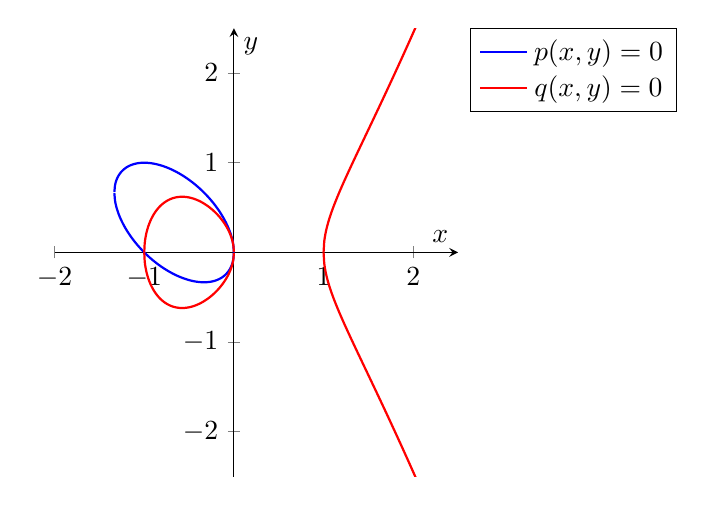
\begin{tikzpicture}
\begin{axis}[
    axis lines=middle,
    xmin=-2, xmax=2.5,
    ymin=-2.5, ymax=2.5,
    xlabel={$x$},
    ylabel={$y$},
    axis equal image, % Para que la elipse no se deforme
    legend pos=outer north east,
    samples=200
]

% Curva p(x,y) = 0 (Elipse)
% Despejando y: y = (-x +/- sqrt(-3x^2 - 4x))/2
% El dominio real es [-4/3, 0]
\addplot [
    blue, 
    thick, 
    domain=-1.3333:0
] {0.5*(-x + sqrt(-3*x^2 - 4*x))};
\addlegendentry{$p(x,y)=0$}

\addplot [
    blue, 
    thick, 
    domain=-1.3333:0,
    forget plot % Para no duplicar en la leyenda
] {0.5*(-x - sqrt(-3*x^2 - 4*x))};

% Curva q(x,y) = 0 (Curva Elíptica)
% Despejando y: y = +/- sqrt(x^3 - x)
% El dominio real es [-1, 0] U [1, infinito)
% Rama 1: [-1, 0]
\addplot [
    red, 
    thick, 
    domain=-1:0
] {sqrt(x^3 - x)};
\addlegendentry{$q(x,y)=0$}

\addplot [
    red, 
    thick, 
    domain=-1:0,
    forget plot
] {-sqrt(x^3 - x)};

% Rama 2: [1, 2.5]
\addplot [
    red, 
    thick, 
    domain=1:2.5,
    forget plot
] {sqrt(x^3 - x)};

\addplot [
    red, 
    thick, 
    domain=1:2.5,
    forget plot
] {-sqrt(x^3 - x)};

\end{axis}
\end{tikzpicture}$$

\end{ejem}
\section{Ra\'ices $n$-\'esimas de la unidad}
Sea $x^n-a\in k[x]$, un radical $n$-\'esimo de $a$ es un $\alpha$ tal que $\alpha^n=0$. 

Si tenemos $\alpha^n=a=\beta^n$ son soluciones de $x^n-a$, al dividir,
$$\frac{\alpha^n}{\beta^n} = \left( \frac{\alpha}{\beta} \right)^n = \frac{a}{a}=1$$
luego $\varepsilon = \frac{\alpha}{\beta}$ es una ra\'iz $n$-\'esima de la unidad, 1, y $\alpha = \varepsilon \beta$ con $\varepsilon=1$, es deicr, toda ra\'iz es un m\'ultiplo de otra por una ra\'iz $n$-\'esima de la unidad.

Consideremos $\mu_n(k) = \{\text{ ra\'ices } n-\text{\'esimas de } 1 \text{ en } k\} = \{\alpha \in k \,/\, \alpha^n=1\}$ que es un sugrupo de $(k^{\times}, \cdot )$. En efecto
$\alpha, \beta \in \mu_n(k) \Rightarrow \alpha \beta^{-1} \in \mu_n(k)$

\begin{ejem}
    $\mu_2(k)=\{1,-1\}$
\end{ejem}
\begin{prop}
    $\mu_n(k)$ es un grupo c\'iclico, $\mu_n(k) = \langle \varepsilon \rangle = \{1,\varepsilon, \varepsilon^2, \ldots, \varepsilon^{n-1}\}$. 
\end{prop}
\begin{defi}
    Una ra\'iz primitiva de la unidad es un generador de $\mu_n(k)$.
\end{defi}
\begin{ejem}
    Si $k=\bb C$, $z=a+bi$, $z^n=1, \, |z^n|=1 \, |z|\in \bb R>0$, $z=\cos \alpha+i \sin \alpha = e^{i\alpha}$, entonces como $z^n = 1 = \cos n\alpha + i \sin n\alpha = 1$, por lo que $n \alpha =0 + \frac{2\pi k}{n}$ para que $\sin =0$ y $\cos =1$. Por tanto, 
    $$\mu_n(\bb C) = \left\{ \cos \frac{2\pi k}{n} + i  \frac{2\pi k}{n} \, /\, k = 0, \ldots, n-1\right\}$$ y $\varepsilon = \cos  \frac{2\pi }{n} + i \sin  \frac{2\pi}{n}$ es una ra\'iz primitva de la unidad.

    De esta forma, $\mu_n(\bb R) = \{1\}$ si $n$ es impar y $\mu_n(\bb R) = \{1,-1\}$ si $n$ es par. 
\end{ejem}
\begin{defi}
    Dada una ra\'iz primitiva $\varepsilon$, llamamos  polinomio ciclot\'omico al $\phi_n(x) \in \bb Q[x]$ de menor grado tal que $\phi_n(\varepsilon)=0$. Adem\'as, en $\bb Q(\varepsilon)$ ya est\'a todos pues $x^n-1 = (x-\varepsilon)(x-\varepsilon^2) \cdots (x-\varepsilon^{n-1}) \quad (x-\varepsilon^n=1)$, y no hace falta extender a $\bb C$, que es un cuerpo mucho m\'as grande.  
\end{defi}
Sea $\alpha \in \mu_n(k)$, es un generado $\iff$ $ord(\alpha)=n$ $\iff$ m\'inimo $k$ tal que $\alpha^{k}=1$, y orden $\alpha$ divide a $|\mu_n(k)|=n$. Supongamos $ord(\alpha)=k$, entonces es una r\'aiz $k$-\'esima primitiva de 1. Por tanto
$$x^n-1 = \prod_{k|n} \phi_k(x)$$
\begin{enumerate}
    \item Supongamos que $n=p$ es primo, no tiene divisores, entonces $x^p-1 =\phi_1(x) \phi_p(x)$ con $\phi_1(x)=x-1$ y entonces $\phi_p(x)=\frac{x^p-1}{x-1} = 1+x+x^2+\cdots +x^{p-1}$.
    \item Si $n=p_1^{\ell_1} \cdots p_s^{\ell_s}$, entonces
    $$\phi_n(x) = \phi_{p_1^{\ell_1}}(x) \cdots \phi_{p_s^{\ell_s}}(x)$$
    porque todo divisor $d|n$, $d=p_1^{k_1}\cdots p_s^{k_s}$ con $k_i \leq \ell_i$. 
    \item Y entonces calculamos $\phi_{p^k}(x) = \phi_{p^{k-1}}(x^p) = \phi_p(x^{p^{k-1}})$ porque $\varepsilon^{p^k}=1 \iff (\varepsilon^p)^{p^{k-1}} = 1$, y ya sabemos calcular $\phi_p(x)$. 
\end{enumerate}
Y el n\'umero de generadores de $\mu_n(k) = $ nº de $s<n$ que son primos con $n =
\phi(n)$.

Para resolver $x^n-a$, $k(\sqrt[n]{a}, \varepsilon)$ tiene todas sus ra\'ices.

Sea $\bb F_q$ un cuerpo finito de $q$ elementos de caracters\'itica $p$, $\bb F_p \subset \bb F_q$ como subcuerpo, y $\dim_{\bb F_p} \bb F_q = n$, y como $\bb F_p$-espacio vectorial tiene una base, $\langle e_1,\ldots, e_n  \rangle = \bb F_q = \{\lambda_1 e_1 + \cdots + \lambda e_n, \, \lambda_i \in \bb F_p\}$ y como $|\bb F_p| = p$, $|\bb F_q| = p^n$.

As\'i pues, $(G=\bb F_q-\{0\}, \cdot)$ es un grupo finito de orden $p^n-1$, luego $0\neq \alpha \in \bb F_q$, y como en general $\alpha^{ord(G)}=1$, $\alpha^{n-1}=1$ y $x^{p^n-1}-1=0$ haciendo que $\bb F_q - \{0\} = \mu_{p^n-1}(\bb F_q)$.

\begin{ejem}
    $\bb F_3(i)$ tiene $3^2 =9$ elementos, que son las ra\'ices de $x^8-1=0$
\end{ejem}
\begin{defi}
    Una $k$-\'algebra es racional si todas sus ra\'ices est\'an en el cuerpo.
\end{defi}
\begin{teo}
    [de Kronecker] Sea $A$ una $k$-\'algebra finita. Existe una extensi\'on finita $k\hookrightarrow L$ de modo que $A \underset{k}{\otimes} L$ es una $L$-\'algebra racional. 
\end{teo}
\begin{dem}
    Por inducci\'on sobre $\dim_k A=n$. 

    Si $n=1$, $A=k$, es racional, solo tiene un punto. 

    Supongamos hasta $n-1$ y vamos a demostrarylo para $n$. Supongamos que $Spec\, A=\{x_1, \ldots, x_s\}, \, s>1$, sabemos que $A = A_1 \times \cdots\times A_s$ siendo $A_i$ \'algebras locales, y $\dim_kA = \dim A_1 + \cdots  + \dim A_s$, y $\dim _k A_1 < \dim A$. Podemos expresar $A = A_1 \times B$ con $\dim B< \dim A$, luego por inducci\'on, existe $k \hookrightarrow L$ tal que $A_1 \underset{k}{\otimes} L$ es racional
    $$A \underset{k}{\otimes} L = (A_1 \underset{k}{\otimes} L) \times (B \underset{k}{\otimes} L)$$
    y $\dim_L B \underset{k}{\otimes} L = \dim_k B$, luego existe una extensi\'on $L \hookrightarrow L'$ de modo que $(B \underset{k}{\otimes} \cancel{L} )\otimes_{\cancel{L}} L' = B \underset{k}{\otimes} L'$ es racional. As\'i, 
    $$A \underset{k}{\otimes} L ' = (A \underset{k}{\otimes} \cancel{L} )\otimes_{\cancel{L}} L' = (A_1 \underset{k}{\otimes} \cancel{L} )\otimes_{\cancel{L}} L' \times B \underset{k}{\otimes} L' = A_1 \underset{k}{\otimes} L' \times B \underset{k}{\otimes} L'$$

    Falta demostrar que si $A$ es una $k$-\'algebra local y racional, entonces $A  \underset{k}{\otimes} L$ es una $L$-\'algebra local y racional. Sea $\m \subset A$ maximal, la sucesi\'on exacta
    $$\bt 0 \rar & \m \rar & A \rar & \modulo{A}{\m}=k \rar & 0 \et$$
    y $A=k \oplus \m$ como espacios vectoriales. Tensorializando sobre $L$,,
    $$A \underset{k}{\otimes} L = k \otimes_{\cancel k} L \oplus \m \underset{k}{\otimes} L = L \oplus \m \underset{k}{\otimes} L $$
    de forma que 
    $$\modulo{(A \underset{k}{\otimes} L )}{\m \underset{k}{\otimes} L} \simeq L$$ luego $\m \underset{k}{\otimes} L\subset A \underset{k}{\otimes} L$ es un ideal maximal, y como $\m \subset A$ son los niltpotentes, $a\in \m$, $a^s = 0 $ haca que 
    $$(a\underset{k}{\otimes}\ell)^s = a^s \underset{k}{\otimes} \ell^s =0 \qquad  a \underset{k}{\otimes} \ell\in \m \underset{k}{\otimes} L$$
    es decir, como $\m \underset{k}{\otimes} L$ contiene a los nilpotentes y $\m \underset{k}{\otimes} L \subset \m$ maximal de $A \underset{k}{\otimes} L$, $A$ sigue siendo local.

    Demostramos cuando $A=A_1$ es local de maximal $\m$ y cuerpo residual $A \overset{\pi}{\longrightarrow}\modulo{A}{\m}=L$, que es una extensi\'on de $k$, de forma que $A \underset{k}{\otimes} L$ es racional, 
    $$\bt \bar \m \rar & A \underset{k}{\otimes} L \rar & L \\[-5mm] & a\otimes \ell \rarmaps & \pi(a) \cdot \ell \\[-5mm] & 1\otimes \ell \rarmaps & \ell \et$$
    de forma que $\ker(\pi \otimes 1)=\bar \m$ es maximal, y $A \underset{k}{\otimes} L$ tiene un punto racional, $A \underset{k}{\otimes} L = A_1\times \cdots $ siendo $A_1$ racional.
\end{dem}
\begin{ejem}
    Sea $\modulo{k[x]}{(p(x))}$, $p(x) = p_1(x)^{\ell_1} \cdots p_s(x)^{\ell_s}$, si $p_1(x)$ es irreducible, $k \subset L=k(\alpha) = \modulo{k[x]}{p_1(x)}$ con $\alpha$ ra\'iz de $p_1(x)$, pero $\modulo{k[x]}{(p(x))} \underset{k}{\otimes} L = \modulo{L[x]}{p(x)}$ ya es racional. Repetimos para todo $p_i$.
    
    Si consideramos $\bb F_3(i) = \modulo{\bb F[x]}{x^2+1}$ como $\bb F_3$-\'algebra, 
    $$\bb F_3 \otimes_{\bb F_3} \bb F_3(i) = \modulo{\bb F_3[x]}{x^2+1} \otimes_{\bb F_3} \bb F_3 = \modulo{\bb F_3(i)}{x^2+1} = \bb F_3(i) \times \bb F_3(i)$$
    con $x\to (i,-i)$, pues $x^2+1=(x-i)(x+i)$, y esta es la descomposic\'on en algebras locales.
\end{ejem}
\begin{prop}
    $\dim_k A = \dim_L(A \underset{k}{\otimes} L)$. Tensorializar mantiene la dimesni\'on y tambi\'en la localidad o no localidad. 
\end{prop}
\begin{obs}
    Sea el automorfismo
    $$\bt A \rar{\tau} & A \\[-5mm] \alpha \rarmaps & \tau(\alpha) \et$$
    y si $\alpha$ es ra\'iz de $p(x)\in k[x]$, $\tau(\alpha)$ tambi\'en lo es, pues $0 = \tau(p(\alpha)) = p(\tau(\alpha))$
\end{obs}
\section{Compuesto de 2 extensiones}
Sean $k \hookrightarrow K_1, k\hookrightarrow K_2$ dos extensiones, el compuesto de estas dos extensiones es una extensi\'on $L$ m\'inima que contiene a $K_1$ y a $K_2$, es decir
$$\bt & K_1  \arrow[hook]{rd}\\ k \arrow[hook]{ru} \arrow[hook]{rd} &  & L\\ & \arrow[hook]{ru}  K_2 \et$$
y al ser m\'inima, no existe $\bar L \subsetneqq L $ tal que $K_1,K_2 \subseteq \bar L$. Se construye como
$$K_1 \underset{k}{\otimes} K_2 = \left\{ \sum_i \lambda_i a_i \otimes b_i \, / \, a_i \in K_1, b_i \in K_2, \lambda_i \in k \right\}$$ 
siendo $K_1,K_2 \subseteq K_1\underset{k}{\otimes} K_2$. $K_1\underset{k}{\otimes} K_2$ puede no ser un cuerpo, si no que $L$ un cuerpo residual, es decir, $L = \modulo{K_1\underset{k}{\otimes} K_2}{\m}$.

Si tenemos $\bb F_q$ el cuerpo finito de $q=p^n$ elementos y $\bb F'_q$ de $q$ elementos, veamos que son isomorfos. Consideremos $L$ un compuesto de ambos, con morfismos $i: \bb F_q \hookrightarrow L$, $j: \bb F'_q \hookrightarrow L$ de forma que $i(\bb F_q) = j(\bb F'_q)$, siendo $i(\bb F_q) =$ra\'ices de $x^q-x$, y $j(\bb F'_q)=$ra\'ices de $x^q-x$, es decir, $\bb F_q \simeq \bb F'_q$ con $j \circ i^{-1}$. 

Dada $k \subset L_1\subset L_2$ una subextensi\'on, $grado_k(L) = \dim_k L$, el $grado_k(L_1)$ divide al $grad_k (L_2)$, de forma que $\dim_k L_2 = \dim_k L_1 \cdot grado_{L_1} L_2$, y si $\dim_k L_1 = n, \, L_1 = \langle e_1, \ldots, e_n\rangle_k$ y $L_2 = \langle v_1, \ldots, v_m \rangle_{L_1}$, $L_2 = \langle e_i \cdot v_j \rangle_{k} (1\leq i \leq n, \, 1\leq j \leq m)$.

Sea $a\in L$, un polinomio m\'inimo de $a$ sobre $k$ es $p(x)\in k[x]$ de grado m\'inimo tal que $0 = p(a)\in L$, es decir, $k[a] \simeq \modulo{k[x]}{p(x)} \subset L $ porque todo anillo \'integro de una $k$-\'algebra finita es un cuerpo. Y $a$ es ra\'iz de $p(x)$. 

Dada una ecuac\'on cuadr\'atica, $p(x) = a_o + a_1x^2 + a_2x^4+\cdots + a_n x^{2n}= 0$, haciendo el cambio $y=x^2$, 
$$q(y)=p(x)=a_o + a_1x+a_2y^2+\cdots + an y^n$$
descendiendo as\'i el grado a la mitad, y si $p(a)=0$, $q(a^2)=p(a) = 0$ y $a^2$ es ra\'iz de $q(y)$, teniendo la subextensi\'on $k \hookrightarrow k(a^2) \hookrightarrow k(a)$, y es una extensi\'on de grado 2, con polinomio m\'inimo $x^2-a^2$. 

Si $p(x)=0$ de ra\'ices $\alpha_1, \ldots, \alpha_n$, $k \hookrightarrow L$ es el cuerpo de descomposici\'on de $p(x) = k(\alpha_1, \ldots, \alpha_n)$ y se tienen las subextensiones $k(\alpha_1) \hookrightarrow k(\alpha_1,\alpha_2) \hookrightarrow \cdots \hookrightarrow  k(\alpha_1, \ldots, \alpha_n)$
con $\modulo{k[x]}{p(x)} \underset{k}{\otimes} L$ es racional, y es el m\'inimo cuerpo donde lo es.

Resolver por radicales es añadir extensiones 
$$k \hookrightarrow k\left( \sqrt[\ell_1]{a_1} \right) \hookrightarrow \cdots \hookrightarrow k\left( \sqrt[\ell_1]{a_1}, \sqrt[\ell_2]{a_2}, \ldots \right) $$ 
y $\alpha_1 = p(\sqrt[\ell_1]{a_1}, \ldots, \sqrt[\ell_s]{a_s})$. En la ecuaci\'on de segundo grado $x^2+ax+b$ es $\alpha=\frac{-a\pm \sqrt{b^2-4ab}}{2a}$. 

Dada una $k$-\'algebra finita $A$, 
$$G=Aut_{k-alg} (A) = \left\{ \tau: A \longrightarrow A\text{ isomorfismos de }k\text{-\'algebras}  \right\}$$ que es grupo con la composici\'on, y se verifica que si $\alpha$ es ra\'iz de $p(x)$, $\tau(\alpha)$ es ra\'iz de $p(x)$, por $\tau(p(x))=p(\tau(\alpha))$. Si $k \to k(\alpha) \simeq \modulo{k[x]}{p(x)} = \{b_o+b_1\alpha + b_s \alpha^s\}$. Rec\'iprocamente, si $\beta \in k(\alpha)$ es una ra\'iz de $p(x)$, $\tau(q(x)) = q(\beta)$ es automorfismo si es ra\'iz ($\tau(b_o + b_1x + \cdots + \alpha_s x^s) = b_o + b_1 \beta + \cdots + b_s \beta^s$), es deicr, las subextensiones son formas de estudiar los cambios variables.

\subsection{Automorfismo de Frobenius}
Si $ch(k)=p (k = \bb F_p)$ y $A$ una $\bb F_p$-\'algebra, existe un automorfismo $\tau: A\longrightarrow A$ que llamaremos de Frobenius, consistente en 
$$\tau(a) = a^p$$
que es un automorfismo por llevar la suma a la suma y el producto al producto:
$$\tau(a+b) = (a+b)^p = a^p + b^p\qquad \tau(ab)= (ab)^p = a^p b^p = \tau(a) \tau(b)$$
y adem\'as por ser isomorfismo, que como es entre espacios vectoriales de la misma dimensi\'on, basta que sea inyectiva o epiyectiva. En efecto, $\ker\tau = \{a\in A\, / \, \tau(a) = a^p =  0\}$ y en $\bb F_p(\alpha)$, $p(x)$ de grado $n$, $\tau(\alpha)=\alpha^p$ es ra\'iz de $p(x)$, y $\tau^2(\alpha) = \alpha^{p^2}$, de forma que $\bb F_q(\alpha)=\bb F_q$ con $q=p^n$, y si hay una ra\'iz, est\'an todas pues son $\alpha^{p^0}, \alpha^p, \alpha^{p^2}, \ldots, \alpha^{p^{n-1}}$. 

\begin{ejem}
    Sea $x^3+x+1$ en $\bb F_2$, no tiene ra\'ices, consideramos entonces $\bb F_2 (\alpha)$ siendo $\alpha$ ra\'iz de $x^3+x+1$ $\bb F_2(\alpha) = \{b_o + b_1 \alpha+b_2 \alpha^2 \, / \, b_1, b_2\in \bb F_2\}$. Y $\alpha, \alpha^2, \alpha^4$ son las ra\'ices, y $\alpha^3+\alpha+1=0 \Rightarrow \alpha^3=\alpha+1$, luego $\alpha^4=\alpha^2+\alpha$. 
\end{ejem}
\section{Separabilidad} 
Intuitivamente, una $k$-\'algebra ser\'a separabale si no tiene puntos repetidos.
\begin{defi}
    Una $k$-\'algebra finita $A$ es $k$-separable si existe una extensi\'on $k \hookrightarrow L$ de modo que $A \underset{k}{\otimes} L$ es $L$-trivializable, es decir, $A \underset{k}{\otimes} L = L^n$. 
\end{defi}
\begin{propis}
\begin{enumerate}
    \item Si $A$ es $k$-separable entonces $A \underset{k}{\otimes} L$ es $L$-separable $\forall k \hookrightarrow L$.
    \begin{dem}
        Supongamos $A \underset{k}{\otimes} L_1 \simeq L_1^n$, de forma que $L_1, L \hookrightarrow L_2$ un compuesto que los contenga, y veamos que $(A \underset{k}{\otimes} L)\otimes_L L_2 = A \otimes L_2$ es trivial, y 
        $$A \underset{k}{\otimes} L_2 = (A \underset{k}{\otimes} L_1) \otimes_{L_1} L_2$$
        $$(L_1 \times \cdots \times L_1)\otimes_{L_1} L_2 = \cancel{L_1} \otimes_{\cancel{L_1}} L_2 \times \cancel{L_1} \otimes_{\cancel{L_1}} L_2  \times c\dots \times \cancel{L_1} \otimes_{\cancel{L_1}} L_2 $$
    \end{dem}
    \item Si $A \underset{k}{\otimes} L$ es $L$-separable, entonces $A$ es $k$-separable.
    \begin{dem}
        Si $L \hookrightarrow \bar L$, $A \underset{k}{\otimes} \bar L = (A \underset{k}{\otimes} L)\otimes_{L} \bar L \simeq \bar L ^n$, trivial
    \end{dem}
\end{enumerate}
\end{propis}
\begin{ejem}
    $\modulo{k[x]}{(p(x))}$ es $k$-separable $\iff$ existe una extensi\'on $k \hookrightarrow L$ con $$\modulo{k[x]}{(p(x))} \underset{k}{\otimes} L \simeq L \times \cdots \times L$$
    $\iff \, p(x)$ tiene todas sus ra\'ices distintas $\iff \, p(x)$ y $p'(x)$ no tienen ra\'ices comunes $\iff\, mcd(p(x), p'(x)) =1$.   
\end{ejem}
\begin{dem}
    Como $\modulo{k[x]}{(p(x))} \underset{k}{\otimes} L  = \modulo{L[x]}{(p(x))}$, y sabmos c\'omo descompone en \'algebras locales, si $p(x) = p_1(x)^{\ell_1} \cdots p_s(x)^{\ell_s}$, 
    $$\modulo{L[x]}{(p(x))} \simeq \modulo{L[x]}{p_1(x)^{\ell_1}} \times \cdots \times \modulo{L[x]}{p_s(x)^{\ell_s}} $$
    con $gr(p_1(x)^{\ell_1})=1$, es decir, $p(x) = (x-\alpha_1) \cdots (x-\alpha_n)$, con $\alpha_ i \neq \alpha_j$ para $i \neq j$.
\end{dem}
\begin{prop}
    [Pregunta corta] Una $k$-\'algebra $A$ es trivial o trivializable $\iff$ es  reducida (producto de cuerpos) y racional (esos cuerpos son $k$, pues tienen todas sus ra\'ices). 
\end{prop}
\begin{defi}
    Una $k$-\'algebra $A$ diremos que es universalmente reducida si para toda extensi\'on $k \hookrightarrow L$, $A\underset{k}{\otimes} L$ es reducida. 
\end{defi}
\begin{prop}
    $A$ es separable $\iff$ $A$ es universalmente reducida. 
\end{prop}
\begin{dem}
    $\Rightarrow)$ Si $A\underset{k}{\otimes} L\simeq L \times \cdots \times L$ es reducida directamente, pues si $A \underset{k}{\otimes} L $ no tiene nilpotentes $A$ tampoco.

    $\Leftarrow)$  Buscamos una \'algebra donde trivialice. Sea $L, k \hookrightarrow L$ tal que $A\underset{k}{\otimes} L$ es racional, como es reducida, $A \underset{k}{\otimes} L = L^n$. 
\end{dem}
\begin{prop}
    C\'omo saber si $A$ es separable. Si $A$ es seprabale y descomponemos en \'algebras locales, $A = A_1 \times \cdots \times A_s$. $A$ es separable $\iff$ $A_i$ es separable $\forall \, i$. 
    \begin{dem} $\Rightarrow)$
        $$(A_1 \underset{k}{\otimes} L )\times \cdots \times (A_s \underset{k}{\otimes} L) \simeq  A\underset{k}{\otimes} L \simeq L^n$$ 
        por lo que por la unicidad de la descomposici\'on, $A_i \underset{k}{\otimes} L \simeq L \times \cdots \times L$. 

        $\Leftarrow) \, A_i \underset{k}{\otimes} L_i \simeq L_i^{n_i}$ con $L_i \hookrightarrow L$ siendo $L$ un compuesto de los $L_i$, entonces 
        $$A \underset{k}{\otimes} L = \prod A_i \underset{k}{\otimes} L =\prod (A_i \underset{k}{\otimes} L_i) \otimes_{L_i} L = \left(\prod L_i \right) \otimes_{L_i} L = \prod L$$
    \end{dem}
\end{prop}
\begin{prop}
    Si $A$ es separable y reducida, $A = K_1 \times \cdots \times K_s$ con $K_i$ cuerpo. 
\end{prop}
\begin{prop}
    Si $a\in A$ es una $k$-\'algebra, diremos que es un elemento $k$-separable si $k[a]\subset A$ es una $k$-\'algebra separable, es decir, $k[a]\simeq \modulo{k[x]}{p(x)}$ con $p(x)$ el polinomio m\'inimo de $a$ $\iff \, mcd(p(x),p'(x))=1$. 
\end{prop}
\begin{dem}
    $k \hookrightarrow K_1$, $k \subset k(a)\subset K_2$. Veamos que si todo elemento es separable, entoces la $k$-\'algebra es separable. Como estamos en un cuerpo, lo demostraremos para este. 
\end{dem}
\begin{prop}
    Sea $k \subset K$ una extensi\'on finita, $K$ es $k$-separable $\iff$ todo elemento de $K$ es separable.
\end{prop}
\begin{dem}
    $\Rightarrow)$ Sea $k(a) \subset K$ es separable porque $k$ es universalmente reducida, entonces al extender $k(a) \underset{k}{\otimes} L \subset K \underset{k}{\otimes} L$ es reducida, entonces una sub\'algebra tambi\'en lo es y entonces $k(a)$ es unviersalmente reducida. 

    $\Leftarrow)$ Supongamos que todo elemento es separable. Por indcuci\'on sobre $\dim_k K$. Si $\dim_k K = 1$, $k=K$ y es trivial.

    Suponemos hasta $n-1$, sea $a\in K, a\nin k$, $k \hookrightarrow L=k(a) \hookrightarrow K$, si $b \in K$, $p(x)\in k[x]$ e sel polinomio m\'inimo de $k$, $p(b)=0$, y si $q(x) \in L[x]$ polinomio m\'inimo sobre $L$ de $b$ divide a $p(x)$, es decir, $p(x) = q(x) \cdot c(x)$. Considerando una extens\'on $L,L\subset L''$, y como trivializa en $L$, tambi\'en en $L''$, es decir $K \underset{k}{\otimes} L''$ es trivializable
    $$K \underset{k}{\otimes} L' \subset K\underset{k}{\otimes} L' \otimes_{L'} L'' = (K \underset{k}{\otimes} L)\otimes_L L ''$$
    y como $(K \underset{k}{\otimes} L)$ es $L$-separable, 
    $$L\underset{k}{\otimes} K \otimes_L L'' = \prod (L'' \underset{k}{\otimes} L) \text{ es reducida}$$
    y por tanto $K \underset{k}{\otimes} L'$ es reducida. 
\end{dem}
\begin{defi}
    Un cuerpo es perfecto si toda extensi\'on finita es separable. 
\end{defi}

Sea $k$ un cuerpo perfecto, $A$ una $k$-\'algebra finita
\begin{prop}
    $A$ es separable $\iff A = K_1 \times \cdots \times K_s$ producto de cuerpos. 
\end{prop}
\begin{dem}
    Ejercicio.
\end{dem}
\begin{ejem}
    Si $k$ es algebraicamente cerrado, entonces es perfecto. 

    Si $ch(k)=0$, entonces es perfecto. 

    Sea $k \hookrightarrow L$ una extensi\'on finita, es separabale $\iff$ todo elemento $a\in L$ es separable, es decir, $k \hookrightarrow k[a] \simeq \modulo{k[x]}{p(x)} \hookrightarrow L$, y $k[a]$ es un cuerpo por ser \'integra y finita, y $p(x)$ es irreducible. Y $\modulo{k[x]}{p(x)}$ es separable $\iff$ $mcd(p(x),p'(x))=1$, y como $p(x)$ es irreducible y por tanto no tiene divisores, la \'unica opci\'on para que $mcd(p(x),p'(x))\neq 1$ es que $p(x)$ divida a $p'(x)$. Sea $p(x) = a_o x^n + a_1 x^{n-1} + \cdots , a_o \neq 0$ y $p'(x)=a_o nx^{n-1} + \cdots, \, a_o n \neq 0 $ de forma que $gr(p'(x))<gr(p(x))$ y el polinomio no puede dividir a su derivada.  

    Si $k$ es finito, entonces $k$ es perfecto, por saber todas las ra\'ices de un $p(x)$. Si $k = \bb F_q$, $q=p^n$ con $p$ primo, sea $\bb F_q \overset{s}{\hookrightarrow} \bb F_{q'}$ una extensi\'on finita, $q'=q^s$, $\bb F_{q'} = \modulo{\bb F_p[x]}{p(x)}$ con $gr(p(x)) = s$ y $p(x)$ irreducible. Solo hay que comprobar que tiene todas sus ra\'ices distintas. Se cumple que $\bb F_q = \{x\,/\,x^{q-1} = 1 \equiv x^q=x \} = \{x^q-x=0\}$, tambi\'en en $\bb F_{q'}$, y consideremos $\tau: \bb F_{q'} \longrightarrow \bb F_{q'}$ el automorfismo de Frobenius, $\tau(\alpha) = \alpha^q$, y si $\alpha \in \bb F_q$, $\tau(\alpha) = \alpha^q = \alpha$, es decir, sobre $\bb F_q$, $\alpha =Id$. Esto nos dice que $\bb F_q(\alpha) = \bb F_{q'}$ y si $\alpha$ es ra\'iz de $p(x)$, $\tau(\alpha)$ es ra\'iz de $p(x)$, y $\tau^2(\alpha)$ es ra\'iz de $p(x)$, y as\'i sucesivamente, y si $gr(p(x))=s$, $\tau^{s-1}(\alpha)$ tambi\'en es ra\'iz, y $\tau^{s}(\alpha) = \alpha^{q^s} = \alpha$. Sea $r<s$, $\tau^r(\alpha) = \tau^{k}(\alpha)$, $\tau^{r-k}(\alpha) = \alpha$, $\tau^r(\alpha) = \alpha$ para $r<s$, de forma que 
    $$\tau^r(q(\alpha)) = q(\tau^r(\alpha)) = q(\alpha) \Rightarrow \tau^r = Id$$
    y entonces tendr\'iamos que $\bb F_{q'} = \{\beta \,/ \, \tau^r(\beta) = \beta, \, \beta^{q^r} = \beta\}$, es decir, se cumple la ecuación $x^{q^r} - x=0$ y $|\bb F_{q'}| =q^s$, y $q^r \geq q^s$ con $r\geq s$, es decir, no hay $s>r$. Entonces en un cuerpo finito todo polinomio m\'inimo verifica que $x^{q'}-x=q(x) = p(x)\cdot s(x)$.
\end{ejem}
\begin{defi}
    Sea $k$ un cuerpo, el cierre algebraico de $k$ es una extensi\'on algebraica $k \hookrightarrow \bar k$ tal que $\bar k$ es algebraicamente cerrado y todo elemento de $\alpha \in \bar k$  verifica ser ra\'iz de alguna ecuaci\'on ($p(x)\in k[x]\, /\, p(\alpha) =0$) o que $k \hookrightarrow k[\alpha] \hookrightarrow \bar k$ es finita.
\end{defi}
\begin{ejem}
    $\bar {\bb C} = \bb C$

    $\bar {\bb R} = \bb C$

    $\bar {\bb Q} = \{\alpha \in \bb C \text{ que son algebraicos sobre } \bb Q\}$, que es un cuerpo, pues $\alpha$ es algebraico si $\bb Q \hookrightarrow \bb Q(\alpha)$ es finita, cogiendo otro $\beta$ algebraico sigue siendo finita. 

    Como $k \hookrightarrow L = k[\alpha ] = \modulo{k[x]}{p(x)}$ una extensi\'on finita, existe $\alpha \in \bar k$ tal que $p(\alpha) = 0$, es decir, $\bar k$ contiene todas las extensiones finitas.

    $\bb F_{p^n} \subset \bb F_{p^r} \, \iff \, n$ divide a $r$. 
\end{ejem}
\begin{teo}
    El cierre algebraico existe. 
\end{teo}
\begin{dem}
    Sea $p(x) \in k[x]$ irreducible, se considera $\displaystyle \bigotimes_k \modulo{k[x]}{p_i(x)}$ con $p_i(x)$ irreducible de forma que $\displaystyle \bigotimes_k \modulo{k[x]}{p_i(x)} = \sum_k e_{i_1} \otimes \cdots \otimes e_{i_n}$ finito, luego $\displaystyle  \modulo{k[x]}{p_i(x)} \hookrightarrow \bigotimes_k \modulo{k[x]}{p_i(x)} \hookrightarrow \bar k$ (todo morfismo entre cuerpos es inyectivo). 
\end{dem}

     Sea $A \simeq k^n$ una $k$-\'algebra trivializable o trivial,
\begin{lem}
    $A$ $k$-\'algebra finita es trivializable $\iff$ $A$ es reducida (producto de cuerpos) y racional (esos cuerpos son $k$). 
\end{lem}
\begin{teo}[Propiedades de las $k$-\'algebras triviales]
    $A$ trivializable, 
    \begin{enumerate}[a)]
        \item  $B \subset A$ es una sub-$k$-\'algebra $\Rightarrow \, B$ es trivializable. 
        \item $A \to B = \modulo{A}{I}$ es un cociente $\Rightarrow \, B$ es trivializable.
        \item Producto directo de trivializables es trivializable
        \item Producto tensorial de trivializables es trivializable
    \end{enumerate}
\end{teo}
\begin{dem}
    \begin{enumerate}[a)]
        \item Se tiene que $B$ es reducida (si $A$ no tiene nilpotentes, una sub\'algebra tampoco), luego descompone $B = K_1 \times \cdots \times K_s \subset A \simeq k^n$. Como cada $K_i \subset K_1 \times \cdots \times K_s$, es morfismo de anillos pero sin elemento unidad, de forma que existe alg\'un $j$ que con la proyecci\'on can\'onica $\pi_j: k^n \longrightarrow k$, que es morfismo de anillos, luego $\pi_j(a) \neq 0$ para alg\'un $j$, de forma que tenemos el morfismo 
        $$\bt K_1 \rar{h} & k \\[-5mm] a \rarmaps & \pi_j(a,0,\ldots,0)  \et$$
        y $\ker h $ es un ideal de $K_1$, pero es un cuerpo, luego como $\ker h\neq K_1$, $\ker h=0$, y tenemos que $h$ es un morfismo inyectivo de $k$-espacios vectoriales, y como $K_1$ es de dim 1, $K_1 \simeq k$ por c\'alculo de dimensiones. Reordenando los t\'erminos, se tiene para todo $i$. 
        \item Como $A=k^n \longrightarrow B = \modulo{A}{I}$, al proyectar, $I = I_1 \times \cdots \times I_s$, siendo $I_i$ ideales de $k$, con $\pi_j(I) = I_j \subset k$, entonces $I_i = 0$ \'o $I_i = k$, de forma que $B = \modulo{k^n}{k^s} \simeq k^{n-s}$, o como puros espacios vectoriales, $k^n = k^s \oplus k^{n-s}$. 
        \item $k^n \times k^m \simeq k^{n+m}$
        \item $k^{n} \underset{k}{\otimes} k^m = \prod k$  por la propiedad distributiva $(A\times B) \underset{k}{\otimes} C = (A\underset{k}{\otimes} C) \times (B \underset{k}{\otimes} C)$, pues 
        $$ (k_1 \times \cdots \times k_n)\underset{k}{\otimes} (k_1 \times \cdots \times k_m) = \prod_{i,j} \cancel{k_i} \otimes_{\cancel{k}} k_j = k^{n+m} $$
    \end{enumerate}
\end{dem}
\begin{teo}[Propiedades de las $k$-\'algebras separables]
    Sea $k \hookrightarrow L$ una extensi\'on que trivializa a $A$, $A \underset{k}{\otimes} L \simeq L^n$,
    \begin{enumerate}[a)]
        \item $B \subset A$ una sub\'algebra $\Rightarrow A\underset{k}{\otimes} L\simeq  L^r$.
        \item $A \longrightarrow B$ cociente $ \Rightarrow B \underset{k}{\otimes} L \simeq L^s$
        \item $A_1,A_2$ son triviales sobre $L$ $\Rightarrow A_1\times A_2$ y $A_1 \underset{k}{\otimes} A_2$ tambi\'en.
    \end{enumerate}
\end{teo}
\begin{dem}
    \begin{enumerate}[a)]
        \item $B\underset{k}{\otimes} L \subset A \underset{k}{\otimes} L$
        \item $A\longrightarrow B$ epiyectivo, $A\underset{k}{\otimes} L \longrightarrow B \underset{k}{\otimes} L $ sigue siendo epiyectivo $\Rightarrow A\underset{k}{\otimes} L \simeq L^s$
        \item $(A_1 \times A_2) \underset{k}{\otimes} L = (A_1 \underset{k}{\otimes} L )\times (A_2 \times L)$

        $(A_1 \underset{k}{\otimes} A_2) \underset{k}{\otimes} L = (A_1 \underset{k}{\otimes} \cancel{L} )\otimes_{\cancel{L}} (A_2 \times L) \Rightarrow (A_1 \underset{k}{\otimes} A_2 \underset{k}{\otimes} L) \simeq  L^m $
    \end{enumerate}
\end{dem}

\begin{ejer}
    [examen] Sea $A = \bb F_2[x,y] / (x+y^2+x^2, x+xy+y^3)$. Las soluciones son f\'aciles de calcular, pues $\bb F_2=\{0,1=-1\}$. Vamos a calcular el espectro y luego vemos su descomposic\'on
    $$\begin{cases}
        x+y^2+x^2 = 0 & \Rightarrow y^2 = x^2+x  \\  x+xy+y^3=0 & \Rightarrow x+xy+(x+x^2) y = x+\cancel{2xy} + x^2y = 0 
    \end{cases}  $$
    $$\Rightarrow x(1+xy) = 0 \Rightarrow \begin{cases}
        x=0, \, y = x^2+x=0 \qquad \qquad x_o=(0,0)\\ x\neq 0, \, 1+xy = 0 \Rightarrow xy=1 \Rightarrow y = \frac{1}{x} \Rightarrow y^2=\frac{1}{x^2} = x^2+x , \, 1=x^3+x^4 \equiv \\ \qquad \qquad  x^4+x^3+1=0
    \end{cases}$$
    y veamos si $x^4+x^3+1$ es irreducible, como no tiene ra\'ices en $\bb F_2$, descompondr\'ia en dos polinomios de grado 2, siendo
    $$x^4+x^3+1 = (x^2+ax+b)(x^2+\bar ax +\bar b)= (x^2+ax+1)(x^2+\bar ax +1)$$
    pues $b\bar b=1$ luego $b=\bar b=1$ y si $a=\bar a =1$, $(x^2+x+1)^2\neq x^4+x^3+1$. Si $a=0$, $\bar a =1$,
    $$(x^2+1)(x^2+x+1) = x^4 + x^3 + x^2 + x^2 + x+ 1 = x^4+x^3+x+1 \neq x^4+x^3+1$$
    y no tenemos m\'as opciones, por lo que $p(x) = x^4+x^3+1$ es irreducible. 

    Sea $\alpha$ ra\'iz de $p(x)$, $\bb F_2 \subset \bb F_2[\alpha]$ una extensi\'on de grado 4, y $x=\alpha, \, y = \alpha^2+\alpha$, y se tienen dos maximales:
    $$\m_{x_o} = (0,0) \qquad \m_{x_1} = \ker p_{\alpha}$$
    siendo $p_{\alpha}$ el morfismo tomar valor 
    $$\bt \m_{x_1} \rar & A \rar & \bb F_2[\alpha] \\[-5mm] & x \rarmaps & \alpha \\[-5mm] & y \rarmaps & \alpha \et$$
    y tenemos la descomposic\'on en \'algebras locales $A=  A_{\m_{x_o}} \times A_{\m_{x_1}}$, entonces en $A_{\m_{x_o}} \simeq \left( \modulo{k[x,y]}{p,q} \right)_{x_o} \overset{x=0}{\simeq} \modulo{k[y]}{(y^2, y^3)} \simeq \modulo{k[y]}{(y^2)}$ no es cuerpo, tiene un nilpotente.
    
    En $A_{\m_{x_1}}$, si $\alpha$ es ra\'iz ($\alpha^r$ tambi\'en, para $r=2,3$), $A_{x_1}\simeq \modulo{k[x]}{x^4+x^3+1} \overset{y=\frac{1}{x}}{\simeq} \bb F_2(\alpha)$.
    
    \underline{No es una \'algebra racional (no tiene todas sus ra\'ices), ni reducida (tiene nilpotentes), ni separable (por no ser racional).}

    Queda calcular un cuerpo donde es racional. 
\end{ejer} 
Sea $A$ una $k$-álgebra separable (si no lo es, es porque tiene nilpotentes y haciendo m\'odulo $mcd(p,p')$ ya es separable), 
    \begin{defi}
        Se llama cuerpo de descomposic\'on de $A$ a una extensi\'on m\'inima $k \hookrightarrow L$ tal que $A \underset{k}{\otimes} L$ es trivial $\iff \, A\underset{k}{\otimes} L $ es racional. 
    \end{defi}
    \begin{ejem}
        Si $A = \modulo{k[x]}{p(x)}$ es seprable, esto es que $p(x)$ tiene todas sus ra\'ices distintas, o que $mcd(p,p')=1$, y $k\hookrightarrow L$ su cuerpo de descomposici\'on es $L= k(\alpha_1, \ldots, \alpha_n)$ donde $\alpha_1, \ldots, \alpha_n$ son ra\'ices de $p(x)$ (fuera de $k$).  As\'i, $A\underset{k}{\otimes} L \simeq \modulo{L[x]}{p(x)} = \modulo{L[x]}{(x-\alpha_1) \cdots (x-\alpha_n)}$ con $\alpha_i \in L$. 
    \end{ejem}
    \begin{defi}
        El cuerpo de descomposici\'on de $p(x)$ (separable) es el cuerpo de descomposici\'on de $\modulo{k[x]}{p(x)}$. 
    \end{defi}\begin{ejem}
        Cuerpo de descomposici\'on de $x^3-2$ sobre $\bb Q$. Sea $\alpha_1 = \sqrt[3]{2}$, $\alpha_i= \varepsilon  \sqrt[3]{2}$ siendo $\varepsilon$ ra\'ices terceras de la unidad. $x^3-2 = (x-1) (x^2+x+1)$. Sea $\varepsilon$ ra\'iz de $x^2+x+1$, $\varepsilon = \frac{-1 \pm \sqrt{2} \cdot i}{2}$, se tiene pues la extensi\'on $\bb Q \subset \bb Q(( \sqrt[3]{2})) \simeq \modulo{\bb Q[x]}{x^3-2} \subset \bb Q( \sqrt[3]{2})(\varepsilon)$, que ya tiene las ra\'ices, y es una extensi\'on de grado 5(no ser\'ia 6?), pues la primera es de grado 3 y la segunda de grado 2. 
    \end{ejem}
